% !TeX root = ../main.tex
\chapter{基于离散扩散模型的语义生成任务迁移方法}
\label{chap:ddcap}
% 这里一个难点是,怎么强调这个事情和CLIP强绑定,
% 也即解释完为什么要套离散版本而不是连续版本之后,
% 需要证明这个事情要和CLIP有关
%%%%%%%
% 一个思路是从Dalle-2出发,Dalle-2可以把Text-Feature Render成Image-Feature for Image-Generation
% 所以我们believe CLIP的Image-Feature可以Read Out Text Annotation;就是强调READ OUT和LiT一样
% 刚好前一章提到的事情就是还不知道怎么把CLIP模型迁移到以图像注释为例的图像生成中去;
% 强调captioning是一种重要的task,所有text生成,比如qa,common sense reasoning本质都是基于caption的一种特殊任务,只需要一个alignment
% 这一章就是借鉴Dalle-2,不过dalle-2两阶段:feature diffusion+raw pixel diffusion
% 这一章直接一阶段出raw text;
% dalle-2是continuous diffusion,我们是discrete diffusion(we also tried continuous diffusion,but not so work)
% 也有一些工作在clip模型后面加ar,这篇文章证明了相比ar来做text generation有一些额外的好处。
% 一个是加速,一个是edit这种特殊任务
%%%%%%%
% 图像字幕任务通常是通过一种逐个解码文本标记的自回归方法来实现的。我们提出了一种基于扩散的字幕模型,称为 DDCap,以实现更大的解码灵活性。与图像生成不同,图像生成中的输出是连续的、冗余的,具有固定长度,而图像标题中的文本是分类的,并且长度不同。因此,天真地将离散扩散模型应用于文本解码效果不佳,如我们的实验所示。为了解决性能差距,我们提出了几种关键技术,包括最佳优先推理、集中注意力掩码、文本长度预测和无图像训练。在没有额外字幕预训练的 COCO 上,它的 CIDEr 分数为 117.8,比受控设置中具有相同结构的自回归基线高 +5.0。在字幕填充任务中,它还执行比自回归基线 (230.3 vs. 203.5) 高 +26.8 的 CIDEr 分数。借助 4M 视觉语言预训练图像和基本大小的模型,我们在 COCO 上达到了 125.1 的 CIDEr 分数,这与最好的成熟自回归框架相比具有竞争力。该代码可在 https://github.com/buxiangzhiren/ DDCap 获取。

%%%%%%%%%%%%%%%%%%%
% 再介绍dalle-2的做法、介绍我们想read-out text,引出扩散模型
% 再介绍dalle-2里的图像扩散模型
% 扩散模型的好处,并行,修改
% 再介绍文本扩散模型的研究,介绍区别,困难和挑战
% 再介绍图像注释任务,图像描述在文本生成任务里的通用性等等(cite llava那些用captioning做pt的)
% 再介绍我们的工作

%%%%%%%%%% 前一章描述
% 虽然本章工作仔细研究了CLIP方法在下游视觉任务,尤其是细粒度视觉任务的迁移表现和改进方法,但如何将CLIP方法迁移到生成式多模态下游任务还不清楚。下一章将以图像注释这一通用任务为主要研究对象,研究CLIP模型实现生成式多模态任务的方法。
%%%%%%%%%%
语言-图像对比学习方法利用互联网图文数据对和实例级对比学习思想驱动模型训练,将视觉表征和语言表征映射到联合空间。CLIP方法得到的视觉表征具有强判别性,被广泛用于零样本开放集合图像识别和图文跨模态检索任务,经过迁移后也可用于目标检测、语义分割、深度估计等下游视觉任务。第\ref{cha:fd}章讨论了如何提升CLIP方法在下游视觉任务上的迁移表现,但未解决语义生成任务的迁移问题。因此,设计合适的迁移方法赋予CLIP方法语义生成能力是本章的研究目标。

\section{引言}
\label{sec:ddcap-intro}
CLIP方法通过对大规模视觉与语义信息进行建模和对齐,具备出色的物体、属性、位置等内容的感知能力,建立起视觉和语言表征间的桥梁,促进图像与文本模态的相互映射和转化。Dall-E 2方法\cite{dall-e2}正是利用了CLIP方法作为跨模态转化的桥梁来完成基于文本的图像生成任务。如图\ref{fig:ddcap-dalle2}所示,对于一段给定的文本,Dall-E 2方法的图像生成过程分为以下两步:
\begin{enumerate}
    \item 利用CLIP方法建立的模态对齐能力进行跨模态表征转化。Dall-E 2方法先利用CLIP方法的语言模型提取给定文本的语言表征,再训练一个基于扩散模型\cite{ddim,ddpm}的先验模型来预测对应的视觉表征。
    \item 将转化好的视觉表征重新映射回像素空间得到原始图像。由于CLIP视觉表征保留了丰富的图像信息,Dall-E 2方法利用一个基于扩散模型的图像解码器将这种视觉表征转化为原始图像。
\end{enumerate}

\begin{figure}
  \centering
  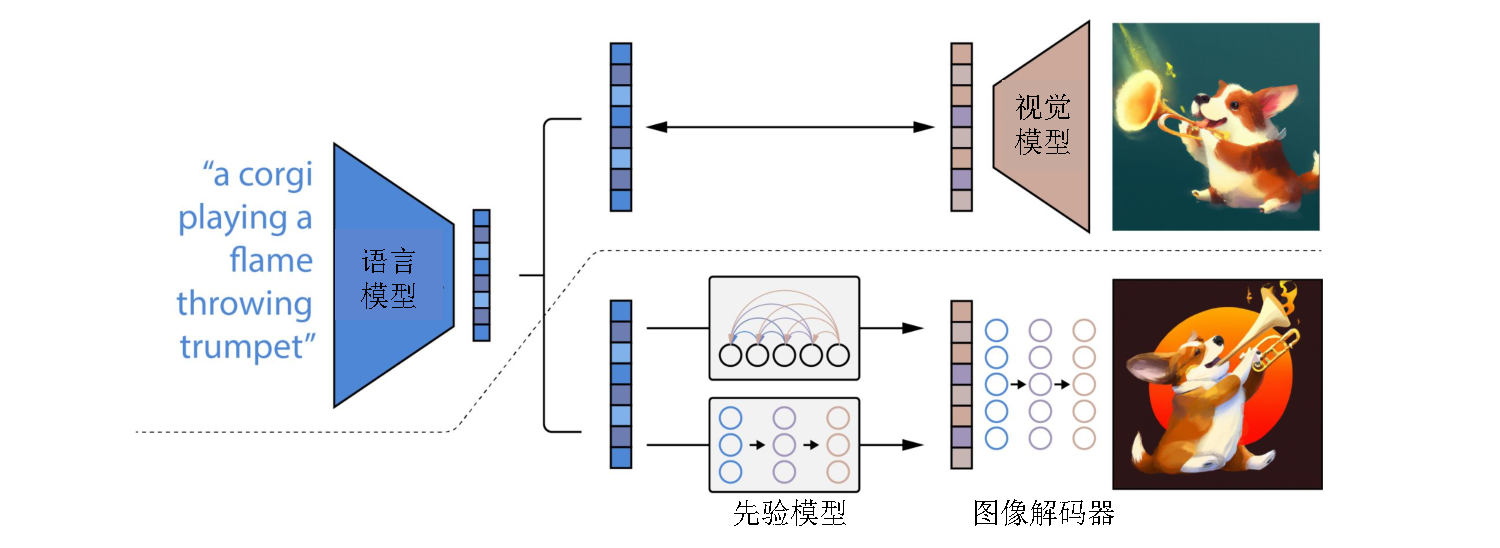
\includegraphics[width=1.0\linewidth]{figures/ddcap-dalle2-v3.pdf}
  % \caption{Dall-E 2方法将CLIP模型的文字表征转化为视觉表征后生成图像}
  \caption{Dall-E 2\cite{dall-e2}方法流程图}
  % 需要辅佐一张图像特征到文本生成的推广
  \label{fig:ddcap-dalle2}
\end{figure}

Dall-E 2方法将CLIP方法成功用于从语言表征到视觉表征的转化,证明CLIP方法得到的多模态表征间有很强的对应关系。这促使本章关注另一个问题:CLIP方法能否将视觉表征转化为语言表征,进而实现基于图像的语义生成任务迁移?值得注意的是,Dall-E 2在上述两个关键转化步骤中均采用了强大的扩散模型作为生成器。扩散模型\cite{ddpm, ddim}已成功用于各类无条件、基于图像类别或基于文本的图像生成任务\cite{beatsgan, glide, latentdiff, imagen},进而产生保真度高、多样性强的图像内容。相比于GAN\cite{gan}等传统生成方法,扩散模型引入迭代生成的思想,可以建模更复杂的数据分布,无需对抗训练而更稳定。相比于自回归的方法,扩散模型可以并行化生成以提高生成效率,并允许模型对已生成结果进行修改,避免了自回归方法因固定生成顺序而导致的误差累积问题。因此扩散模型已经逐渐成为图像生成任务的主流方法,并在现实场景中得到了大规模应用\cite{latentdiff, dall-e2}。

\begin{figure}
  \centering
  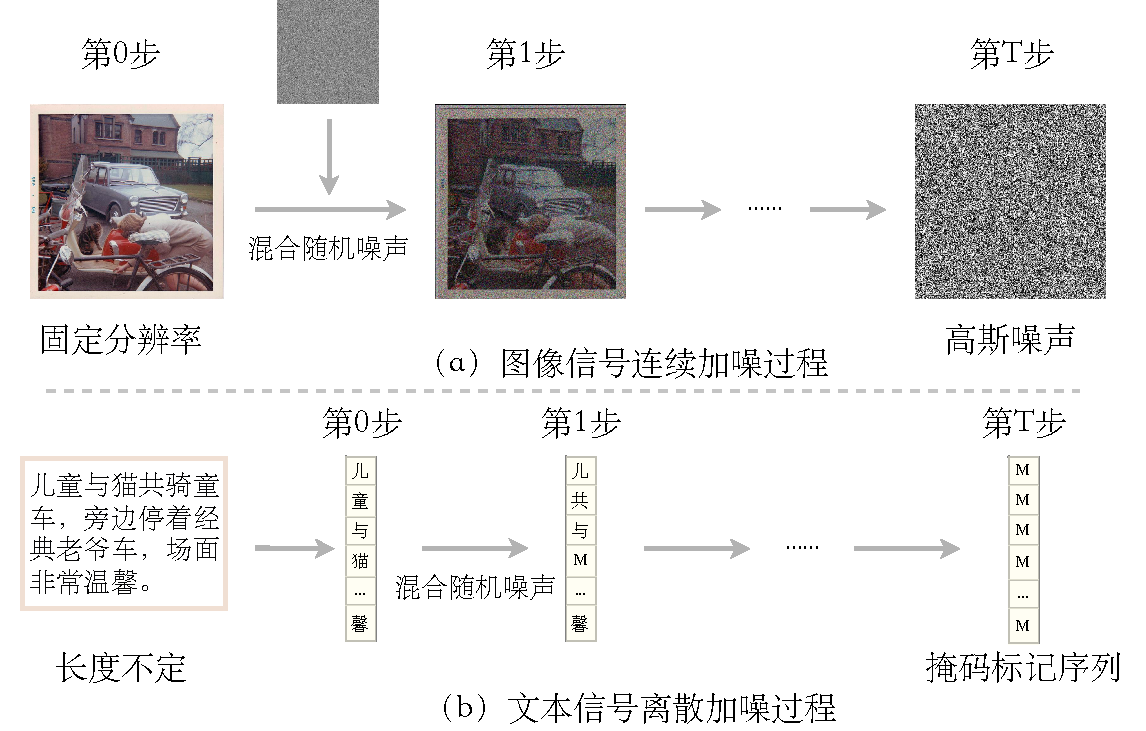
\includegraphics[width=1.0\linewidth]{figures/ddcap-img-text-diff.pdf}
  \caption{图像生成任务和文本生成任务在加噪过程中的区别}
    % 图 2.(a) 图像生成:噪声是连续的、冗余的,具有固定的长度 (b) 文本生成:噪声是分类的,而且很短,长度各不相同。
  \label{fig:ddcap-img-text-diff}
\end{figure}


然而,目前已有的研究中尚无直接有效的方法将扩散模型应用于基于图像的文本生成任务\cite{karpathy2015deep, vinyals2015show}。如图\ref{fig:ddcap-img-text-diff}所示,站在生成任务的视角,图像信号与文本信号存在几项固有的区别:
\begin{itemize}
    \item 信号在连续性和冗余性方面的区别。在图像生成任务中,因为输出图像除主体部分外往往包含信息密度更低的背景内容,因此,图像信号通常表现为具有连续且高度冗余特性。但在文本生成任务中,输出文本是离散且信息精炼的,通常不包含与图像内容无关的冗余信息。
    \item 信号序列长度可变性的区别。图像生成任务具有固定的输出分辨率,通常为$32^2$、$64^2$等固定尺寸。而且图像信号的连续特性使得调整图像分辨率相对容易实现\cite{dall-e2,super-resolution}。而文本生成任务则恰好相反,不同图像对应的文本信息长度多样。常见任务的文本长度在10到50之间不等。但文本信号的离散性使得对其长度进行类似图像分辨率调整的操作非常困难。
    \item 噪声建模方式的区别:扩散模型的推理过程是一个在输入中反复添加噪声并进行去噪预测的循环过程。由于图像信号的连续性和冗余性,在图像信号中添加噪声后,各个像素仍保有部分原始信息。因此模型可相对容易地利用信噪比较高的邻近像素信息进行预测。但在离散的文本信号中添加噪声后,正确文字可能会被直接替换为错误文字,此时单个文字的原始信息几乎完全丢失。因此对于文本生成任务而言,扩散模型的推理过程也需要特殊设计。
\end{itemize}

% 由文本扩散模型的困难介绍文本扩散模型的好处,以及引出我们为什么选择了图像注释任务
% 虽然利用扩散模型将CLIP的图像特征转化为文本特征仍有一定挑战,但由于扩散模型提供了并行生成的可能性,允许对上下文信息同时建模,并天然支持对中间结果进行修改,在行为自由度上和人类更为相似,这些优势促使本章对此进一步探索。
因此,本章系统地研究了基于扩散模型将CLIP方法迁移至下游语义生成任务的方法。前期实验表明,连续扩散模型在文本生成任务上表现欠佳,与主流自回归方法\cite{OSCAR,VinVL,UFO,ViTCap,SimVLM,GIT}相比性能差距明显。基于上述对文本信号离散特性的分析,本章主要讨论了离散扩散模型\cite{VQ-diffusion},并提出了更适合文本生成任务训练和推理过程的DDCap方法。在训练方面,DDCap方法引入长度预测任务,先预测待生成文本长度再进行推理,从而灵活适应不同长度的文本信号。考虑到文本的离散性和信息密集特性,DDCap方法在模型自注意力层中添加集中注意力掩码模块,使模型自适应地关注信息量更大的文本位置。在推理方面,DDCap方法设计了最佳优先推理策略,在每个扩散去噪步骤中保持已恢复的置信度最高的$K_{t}$个文本标记不变,避免它们在后续重新加噪过程中被改变。其中$K_{t}$值设置为待预测文本长度与推理步数的比值,使得模型在每一步中输出的信息量基本均匀。最后,受图像生成模型中无分类器引导方法\cite{glide}启发,DDCap方法引入无图像引导文本生成训练策略从而增强模型鲁棒性。具体而言,DDCap方法在训练过程中随机丢弃部分样本的图像输入以促使模型学习文本先验知识。在推理时,DDCap方法对基于文本先验知识的输出和以图像内容为条件的输出进行加权组合,获得与图像内容更相关的生成结果。
% 首先在训练方面,DDCap方法提出引入一个长度预测任务,实现先预测待生成文本长度,再进行推理过程的做法,从而更灵活地适应不同长度的文本信号。考虑到文本信号的离散特性和信息密集特性,DDCap方法提出在模型自注意力层中添加集中注意力掩码模块,以便模型自适应地专注于信息量更大的文本位置。其次在推理方面,DDCap方法中设计了一种称为最佳优先的推理策略。该推理方法保持每个扩散去噪步骤中恢复的最佳$K_{t}$个标记不变,使其不会在后续的重新加噪步骤中被替换为其他文本内容。
% % 换句话说,在每个扩散去噪步骤中定期选择一组标记固定下来不再改变,并在加噪步骤中,只对未标记为固定的标记集合添加噪声。
% 其中每个去噪步骤中保持的标记数目$K_{t}$大致设置为长度预测任务输出的文本长度与推理过程步数的比值。最后,受图像生成模型的无分类器引导方法\cite{glide}启发,DDCap方法提出引入无图像训练的文本生成方法以增强模型的鲁棒性。具体而言,DDCap方法在训练过程中会随机选择一些训练样本,将其图像输入丢弃后预测对应文本内容,以强制模型学习文本的先验知识。在推理过程中,DDCap方法可以对基于文本先验的输出和基于图像内容的输出进行加权组合,从而获得与图像内容联系更紧密的文本生成结果。

% 本章选取了最具有代表性的图像注释任务(Image Captioning)\cite{karpathy2015deep, vinyals2015show}作为主要研究对象。
% 图像注释任务是一种特殊的基于图像的文本生成任务,可作为辅助阅读手段,具有较强的现实意义。
% 同时,图像注释任务被认为是各类下游多模态任务的通用代理任务\cite{llava},如图文问答、物体定位等,因此提高图像注释能力对其他任务也有帮助。
% 此外,图像注释任务能够成为自动生成互联网替代文本的一种方式,进而反过来拓宽CLIP预训练数据的来源,从而形成数据飞轮\cite{blip-2}。

本章在图像描述生成任务\cite{karpathy2015deep, vinyals2015show}中验证DDCap方法,表明离散扩散模型能够有效地将CLIP视觉表征转化为语义输出,从而实现语义生成任务的迁移。在不失一般性的前提下,本章使用最常用的OpenAI CLIP\cite{radford2021learning}模型作为待迁移模型。在包含1000万图文对的数据集上对CLIP模型进行迁移训练后,DDCap方法在MSCOCO数据集\cite{chen2015microsoft}上取得了125.1的CIDEr-D分数\cite{cider},与多个先进自回归方法\cite{OSCAR,VinVL,UFO,ViTCap}结果相当,远优于基于连续扩散模型的迁移方法。
此外,这种基于离散扩散模型的语义生成任务迁移方法使得模型能够在生成图像描述过程中同时考虑上下文语境,并具备对已生成内容进行修改的能力。因此,本章还提出了更适合人机交互场景的描述修改任务,即删除已生成图像描述中的所有形容词,要求模型根据上下文重新预测被删除的内容,并使用CLIPScore\cite{CLIPScore}方法评估修改前后的图像描述与图像间的语义匹配程度。实验证明基于离散扩散模型的迁移方法相比自回归方法更能把握细微语义变化,在图像描述修改任务中表现更佳。

% 本章将DDCap方法在图像描述生成任务\cite{karpathy2015deep, vinyals2015show}中进行了验证,证明了利用离散扩散模型将CLIP模型的视觉表征转化为语义输出,并实现语义生成任务迁移的可行性。
% DDCap方法使用含有1000万个图像-描述对的数据集对CLIP模型进行微调后,在MSCOCO数据集\cite{chen2015microsoft}的图像描述生成任务上取得125.1的CIDEr-D\cite{cider}分数。这一结果与一些最先进的自回归模型\cite{OSCAR,VinVL,UFO,ViTCap}结果相当。
% 此外,这种基于离散扩散模型的语义生成任务迁移方法可以使得模型在生成图像描述时同时考虑上文和下文,并赋予了模型对已生成内容进行修改的能力。
% 因此,本章还提出了一项更适合人机交互场景的描述修改任务。在此任务中删除了已生成图像描述中的所有形容词,要求模型根据上下文去重新预测被删除的内容,并使用CLIP分数\cite{CLIPScore}来评估修改前后内容间的语义匹配程度。实验证明基于离散扩散模型微调的模型相比于基于自回归方法微调的模型更能把握细微的语义变化,并在描述修改任务中表现更佳。

综上所述,本章的主要内容安排如下:
\begin{itemize}
    \item 第\ref{sec:ddcap-intro}节讨论了图像生成领域中的扩散模型,以及文本信号区别于图像信号的关键特性:离散性、低冗余性、序列长度可变性。
    \item 第\ref{sec:ddcap-method-all}节介绍了用于语义生成迁移的离散扩散模型基本思想,以及针对文本信号特性设计的训练与推理方法:集中注意力掩码模块、长度预测任务和最佳优先推理策略,以及无图像引导文本生成训练策略。
    \item 第\ref{sec:ddcap-result}节介绍了本章的实验设置、评测指标和实验结果,并介绍了图像描述修改任务设置与测试结果。
    \item 第\ref{sec:ddcap-summary}节对本章内容进行了总结。
\end{itemize}

% 因此,本文的贡献总结为
% • 我们是第一个将离散扩散模型应用于图像描述的公司,并提供了第一个证据,证明扩散模型可以达到与最好的、完善的自回归模型相比的竞争性能。
% • 我们提出了四个关键设计:(i) 长度预测用于处理文本生成中的可变长度问题;(ii) 集中注意力掩码用于提取紧凑的文本信息,而不会受到不需要的噪音的干扰;(iii) 提出了最佳优先推理以减少污染正确生成的令牌的机会;(iiii) 无图像训练,以平衡文本先验和图像条件中的信息。
% • 我们进一步展示了离散扩散模型在标题填充任务中的优势。

% 本文的其余部分组织如下。我们在第 2 节中总结了相关工作。第 3 节提出了拟议的 DDCap 模型的细节。第 4 节报告了大量的实验结果,包括定量和定性讨论。我们最后在第 5 节中得出结论。


\section{研究方法}
\label{sec:ddcap-method-all}
本节介绍了基于离散扩散模型的语义生成任务迁移方法DDCap。第\ref{sec:ddcap-method}节首先讨论了将离散扩散模型应用于图像描述生成任务的基本思想。第\ref{sec:ddcap-key-design}节详细阐述了针对文本信号的离散性、低冗余性和序列长度可变性设计的关键训练和推理方法。

% 本节详细介绍了基于离散扩散模型实现CLIP模型在语义生成任务上微调的DDCap方法。
% 与当前主流的自回归方法相比,这种方法具有更大的解码灵活性。例如,这种方法允许同时预测多个标记,而不是逐个预测,前文标记也可以依赖后文标记进行生成并修改,而不是仅只允许按阅读顺序进行生成。
% 第\ref{sec:ddcap-method}节首先介绍了将离散扩散模型应用于图像描述生成任务的基本思想。第\ref{sec:ddcap-key-design}节接着详细介绍了多种针对文本信号的离散性、冗余特性、序列长度可变性设计的训练和推理方法,对提高性能起到了关键作用。

\subsection{离散扩散模型的基本思想}
\label{sec:ddcap-method}
连续扩散模型在每个图像像素上单独施加连续高斯噪声,因此可以精确且连续控制各元素的噪声强度。与连续扩散模型不同,离散扩散模型则在实例级别控制整体噪声强度,通过对单个元素进行掩码或替换操作实施加噪过程。对标记化后的文本序列而言,离散扩散模型通过将文本标记替换为掩码标记[\texttt{MASK}]或其他随机文本标记来实现加噪。当文本标记被替换为随机标记时,该输入元素的信噪比显著降低,而当该文本标记被进一步被替换为掩码标记时,输入元素的原始信息几乎完全丢失,仅作占位符用途。因此,受文本信号离散性特点影响,离散扩散模型无法连续调节单个输入元素的噪声强度,而是通过控制掩码标记比例来调节整个输入序列的噪声水平。

% 连续扩散模型将连续高斯噪声单独施加在每个图像像素之上,因此输入模型的每个元素都可以连续控制不同的噪声强度。与连续扩散模型不同,离散扩散模型通常在实例级别实行加噪过程,以控制其整体噪声强度。对单个元素而言,离散噪声通常以掩码或替换的形式实现。对标记化后的文本序列而言,离散扩散模型使用掩码标记[\texttt{MASK}]或其他随机正常文本标记替换当前的文本标记作为加噪方法。
% 一旦当前的文本标记被替换为其他随机的正常文本标记,该输入元素的信噪比就降到了很低的水平。如果该文本标记被进一步替换为掩码标记,则此时该输入元素的原始信息几乎完全丢失,只起到了占位符的作用。
% 因此,离散扩散模型无法连续控制单个输入元素的噪声强度,而是通过控制掩码标记比例来控制输入序列的整体噪声水平。
% \todo{目前的符号里混杂了标记x和标记序列x,也混合了gt的x和预测的$\hat{x}$}

\paragraph{加噪过程} 本章使用GPT-2模型的分词器\cite{gpt2}将图像描述文本转化为文本标记序列。图像描述中的每个文本标记记作$x$,是一个有5万多种可能取值的离散变量。

离散扩散模型的加噪过程可以描述为一个一阶马尔可夫过程。每个离散的马尔可夫状态跳转都在逐步增加文本标记序列的噪声水平。将对文本标记$x$加噪$t$步后得到的标记表示为$x_{t}$,初始状态$x_0=x$。在每一加噪步中,正常文本标记都有一定概率转换为掩码标记,而掩码标记作为特殊的吸收状态,一旦转变为此状态将不再改变。因此,如果$x_{t-1}$不是掩码标记,那么在第$t$个加噪步中$x_{t-1}$到$x_t$的状态转移概率定义为:
% 离散扩散模型的加噪过程可以被认为是一个仅依赖前一步状态的马尔可夫过程,逐步地增加文本标记序列的噪声水平。将对文本标记$x$加噪了$t$步得到的标记表示为$x_{t}$,可以得到$x_0=x$。
% 在每一个加噪步中,任何正常文本标记都有一定概率被转换成掩码标记。而掩码标记是一种特殊的吸收状态。任何已经转变为掩码标记的$x_{t}$将一直停留在掩码标记状态。因此,如果$x_{t-1}$还不是掩码标记,那么在第$t$个加噪步中$x_{t-1}$的状态转移概率定义为:
\begin{equation}
    q(x_t | x_{t - 1}\neq\texttt{[MASK]}) = 
    \begin{cases}
    \alpha_t, & x_t = x_{t - 1} \\
    \gamma_t, & x_t = \texttt{[MASK]} \\
    1 - \alpha_t - \gamma_t, & \text{其他情况}.
    \end{cases}
    \label{eq:iclip-q-nonmask}
\end{equation}

具体而言,在第$t$个加噪步中,$x_{t-1}$有$\alpha_{t}$的概率保持原文本标记不变,有$\gamma_{t}$的概率转换为掩码标记,还有$\beta_{t}=1-\alpha_{t}-\gamma_{t}$的概率随机转换为词汇表中其他文本标记,这些不同文本标记的转移概率相同。若$x_{t-1}$已经是掩码标记[\texttt{MASK}],在第$t$个加噪步中$x_{t-1}$到$x_t$的状态转移概率定义为:
% 具体而言,在第$t$个加噪步中,$x_{t-1}$有$\alpha_{t}$的概率保持原文本标记不变,有$\gamma_{t}$的概率被转换成掩码标记,同时还有$\beta_{t}=1-\alpha_{t}-\gamma_{t}$的概率被随机转换成词汇表中的其他文本标记。
% 如果$x_{t-1}$已经是掩码标记[\texttt{MASK}],由于其是一个吸收状态,在第$t$个加噪步中$x_{t-1}$的状态转移概率定义为:
\begin{align}
    q(x_t | x_{t - 1} = \texttt{[MASK]}) = 
    \begin{cases}
    1,& x_t =\texttt{[MASK]} \\
    0,& \text{其他情况}.
    \end{cases}
    \label{eq:iclip-q-mask}
\end{align}

当反复对文本序列施加公式\eqref{eq:iclip-q-nonmask}和\eqref{eq:iclip-q-mask}中的加噪过程,且总步数$T$足够大时,所有文本标记最终都会转变为掩码标记。这种状态也是推理过程的开始状态。
% 通过对整个文本序列反复施加公式\eqref{eq:iclip-q-nonmask}和公式\eqref{eq:iclip-q-mask}中描述的加噪过程,只需要总步数$T$足够大,最终所有文本标记都会转变为掩码标记。% 这也是推理阶段的起点。

% \begin{figure}
%   \centering
%   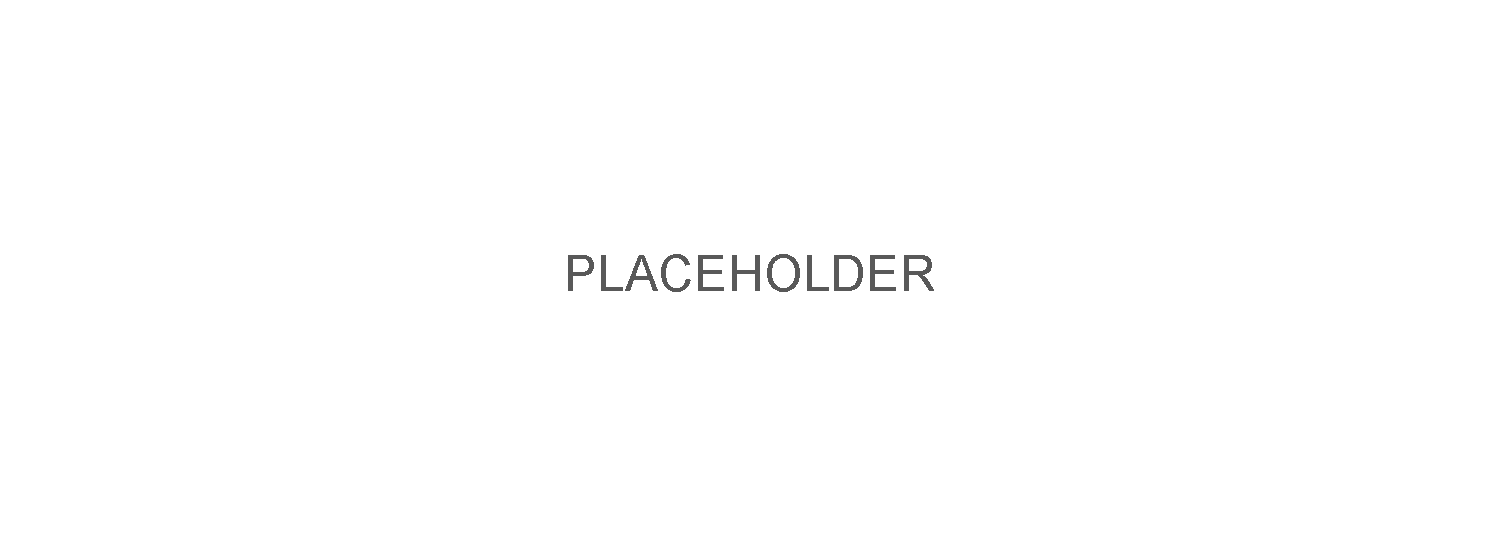
\includegraphics[width=1.0\linewidth]{figures/placeholder.pdf}
%   \caption{DDCap模型结构示意图}
%   % image encoder; decoder (cross-attn) + time step
%   \label{fig:ddcap-arch}
% \end{figure}

\paragraph{去噪过程} 
去噪过程是加噪过程的逆过程。离散扩散模型的去噪过程从全掩码标记序列开始,逐步施加去噪步以恢复原始输入信号,最终得到完整的图像描述。因此,离散扩散模型训练的主要目标即是对该去噪过程建模,表示为:
\begin{equation}
\max_{\theta} p_{\theta}(x_{t-1} | x_{t}, y),
  \label{eq:ddcap-target}
\end{equation}
其中$y$为从CLIP视觉表征,$\theta$为待训练的模型参数。

本章采用Transformer\cite{Transformer}模型结构作为模型$\theta$,以建模文本序列的去噪过程。为了以视觉表征$y$为条件输出$x_{t-1}$,本章考虑两种方式:
\begin{itemize}
    \item 在输入序列维度上拼接视觉表征$y$与待去噪文本序列$x_{t}$,并用Transformer模型结构的自注意力机制进行建模;
    \item 用交叉注意力机制,将视觉表征$y$的信息逐层融合进待去噪文本序列$x_{t}$中;
\end{itemize}
本章实验采用第二种建模方式,既避免了视觉表征与文本序列位置编码融合的问题,又增强了待去噪文本序列对视觉表征的关注度。
% 整体结构示意图如图\ref{fig:ddcap-arch}所示。

为在不同去噪步$t$时激发不同的模型行为$\theta_t$,本章遵循图像生成扩散模型\cite{VQ-diffusion}的一般做法。该做法将去噪步$t$信息编码为正余弦位置嵌入后,注入模型的自适应层归一化模块\cite{adaln}中,进而改变该模块对特征的缩放和偏移参数,达到激发不同模型行为的目的。模型不同维度$i$的正余弦位置嵌入方式如下:
\begin{equation}
    \text{PE}_{i} = \begin{cases}
    \sin(\frac{p}{10000^{2i/d_{\text{model}}}}), i < \frac{d_{\text{model}}}{2} \\
    \cos(\frac{p}{10000^{2i/d_{\text{model}}}}), i \ge \frac{d_{\text{model}}}{2},
    \end{cases}
    % emb = self.linear(self.silu(self.emb(timestep))).unsqueeze(1)
    % scale, shift = torch.chunk(emb, 2, dim=2)
    % x = self.layernorm(x) * (1 + scale) + shift
    \label{eq:ddcap-t}
\end{equation}
其中$p = t/T\times \text{step}_{\text{scale}}$,而$d_{\text{model}}$是模型隐藏层维度。$\text{step}_{\text{scale}}$作为调整正余弦函数周期的超参数,其值越大,模型在不同去噪步间的行为差异越显著;反之,模型行为则更为一致。
% 其中$d_{\text{model}}$是模型隐藏层维度,$p = t/T\times \text{step}_{\text{scale}}$。
% $\text{step}_{\text{scale}}$是一个调整正余弦函数周期的超参数。越大的$\text{step}_{\text{scale}}$值会放大模型在不同去噪步$t$之间的行为差异,越小的值则会使得模型在不同去噪步$t$间的行为更一致。
%在本章实验中一般设$\text{step}_{\text{scale}}$为8000。

\paragraph{训练过程} 训练过程的核心是使模型$\theta_t$对第$t$步的去噪过程进行建模。连续扩散模型通常采用预测噪声形式为学习目标,而离散扩散模型由于在句子级别控制噪声强度并通过掩码或替换策略实施加噪过程,无法直接将单元素噪声转化为可学习目标。受已有工作\cite{structddm}启发,DDCap方法以直接预测原始文本标记$x_{0}$为学习目标,损失函数为:
% 训练过程本质是驱动模型$\theta_t$对去噪过程进行建模。在连续扩散模型中,去噪过程的学习目标通常是预测噪声形式,而离散扩散模型通过掩码或替换策略在句子级别控制不同的噪声强度,因此无法将单元素的噪声转化成可学习目标。
% 受已有工作\cite{structddm}启发,DDCap方法的实际训练目标为直接预测原始文本标记$x_{0}$。损失函数形式如下:
\begin{equation}
\mathcal{L}=-\log p_{\theta_t}(x_0 | x_t, y).
\end{equation}

% 而公式\eqref{eq:ddcap-target}中描述的去噪过程建模目标,可以通过如下重参数化技巧\cite{VQ-diffusion}得到:
公式\eqref{eq:ddcap-target}中的去噪过程建模目标可通过重参数化技巧\cite{VQ-diffusion}转化得到:
\begin{equation}
    p_{\theta_t}(x_{t-1} | x_{t}, y)=\sum_{\hat{x}_0=1}^{V}q(x_{t-1}|x_{t},\hat{x}_0)p_{\theta_t}(\hat{x}_0 | x_{t}, y),
\end{equation}
其中$V$表示所有可能的文本标记总数,$\hat{x}_0$表示模型基于当前第$t$步输入对原始文本标记$x_{0}$的预测结果。而$q(x_{t-1}|x_{t},\hat{x}_0)$可通过贝叶斯公式求得:
\begin{equation}
    q(x_{t-1}|x_{t},\hat{x}_0)=\frac{q(x_{t}|x_{t-1},\hat{x}_0)q(x_{t-1}|\hat{x}_0)}{q(x_{t}|\hat{x}_0)}=\frac{q(x_{t}|x_{t-1})q(x_{t-1}|\hat{x}_0)}{q(x_{t}|\hat{x}_0)}.
\end{equation}

DDCap方法的训练过程如图\ref{fig:ddcap-train-inference}的左侧部分所示。

\paragraph{推理过程} 离散扩散模型的推理过程从一个完全由掩码标记[\texttt{MASK}]组成的序列$x_{T}$开始,应用模型$\theta_{T}$习得的去噪过程得到预测结果$\hat{x}_{0}$,并对其重新加噪得到$x_{T-1}$。循环往复$T$步之后,即可得到最终预测结果。因此,与自回归方法在序列维度进行迭代不同,离散扩散模型在噪声强度维度进行迭代。

从$x_{t}$推理出$x_{t-1}$的单步去噪过程计算如下:首先,利用训练好的模型$\theta_t$根据CLIP视觉表征$y$和当前文本序列通过$p_{\theta_t}(x_{0} | x_{t}, y)$估计出$\hat{x}_{0}$;其次,利用加噪过程的马尔可夫性推导出$x_{t-1}$的分布并进行采样。具体公式为:
\begin{equation}
    q(x_{t-1} | \hat{x}_{0})=\prod \limits_{i=1}^{t-2} q(x_{i+1} | x_i)\cdot q(x_1 | \hat{x}_{0}).
\end{equation}

由于在离散扩散模型推理过程的每一中间步中,模型均给出了基于当前噪声输入的原始文本序列预测$\hat{x}_{0}$。因此,离散扩散模型支持通过快速采样方式加速推理过程,从而在$T$步内获得较准确的预测结果。DDCap方法的推理过程如图\ref{fig:ddcap-train-inference}的右侧部分所示。
% 离散扩散模型通过不断的加噪和去噪的循环,在$T$步之后得到最终预测结果$\hat{x}_{0}$。由于每一个中间步中,模型均给出了基于当前噪声输入下对原始文本序列的预测结果,因此离散扩散模型允许通过一些快速采样的方式对推理过程进行加速,使其在小于$T$步之内得到较为准确的预测结果。DDCap方法的推理过程如图\ref{fig:ddcap-train-inference}的右侧部分所示。

\begin{figure}
  \centering
  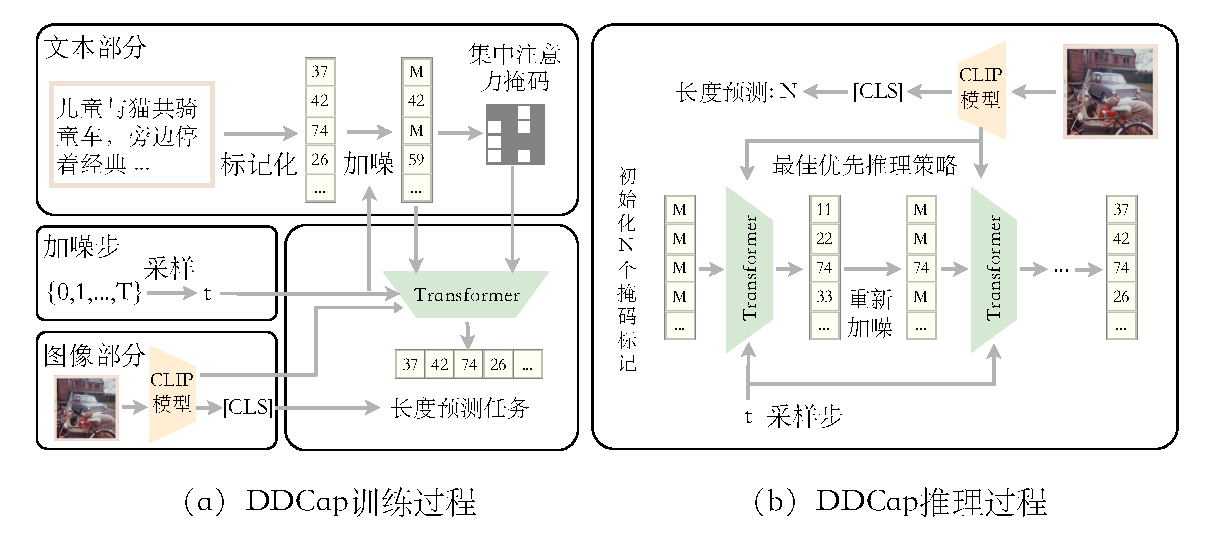
\includegraphics[width=1.0\linewidth]{figures/ddcap-train-inference.pdf}
  \caption{DDCap方法训练过程和推理过程示意图}
  % image encoder; decoder (cross-attn) + time step
  \label{fig:ddcap-train-inference}
\end{figure}

%%%%%%%%%%%%
\subsection{针对文本信号特性的关键设计}
\label{sec:ddcap-key-design}
前期实验表明,仅采用上述简单设计时,离散扩散模型在语义生成任务迁移性能上远弱于自回归方法,难以生成完整且有意义的图像描述。根据第\ref{sec:ddcap-intro}节对图像和文本信号特性的分析,这是因为文本生成与图像生成任务存在显著差异,所以将图像生成任务的离散扩散模型直接用于文本生成任务无法取得较好的迁移性能。
首先,待生成文本长度多变,而图像分辨率通常固定。其次,文本信息较为紧凑,单个文本标记的改动可能导致整段文本意义完全改变或表意不明,而图像中的冗余信息较多,相邻像素间的连续性可提供互证信息。此外,由于离散扩散模型中引入掩码标记[\texttt{MASK}]和标记替换策略实施加噪过程,因此文本标记间的语义离散性使得单个输入元素的噪声强度近似为阶跃函数:一旦该文本标记被替换或掩码,几乎无法保留任何原始信息。而在图像生成任务中,图像解码器提供一定的冗余性,使得单个标记承载的信息可通过其他标记所反映。基于这些观察,本节提出四种针对文本生成任务的关键设计:长度预测任务、集中注意力掩码模块、最佳优先推理策略和无图像引导文本生成训练策略。

% 前期实验发现,仅通过上述设计的简单实现,离散扩散模型相比于自回归模型方法在语义生成任务迁移上表现较弱,几乎无法生成完整有意义的图像描述。
% 根据第\ref{sec:ddcap-intro}节中的对图像信号和文本信号特性的分析,文本生成任务与图像生成任务有相当大的不同。
% 首先,待生成文本的长度多变,而待生成图像的分辨率通常是固定的。
% 同时,文本中的信息比较紧凑,单个文本标记改动之后可能会使得整段文本具有截然不同的意思或出现表意不明的现象,但是图像中的冗余信息较多,不同像素之间由于邻域内的连续性可以提供互相印证的信息。
% 此外,由于离散扩散模型中引入掩码标记[\texttt{MASK}]和标记替换来构造噪声,因此不同文本标记之间语义的离散性导致对单个文本标记而言,其噪声强度近似是一个阶跃函数:一旦被替换为别的文本标记或掩码标记,该文本标记上的信噪比接近于0。但是对于基于离散扩散模型的图像生成任务而言,后续的图像解码器提供了一定的冗余性,使得当前图像标记承载的信息可以通过别处的图像标记所反映。
% % 每个像素上的噪声强度可以被连续控制,不会出现完全不提供信息的情况。
% 受这些观察启发,本节提出了以下四种针对文本生成任务的关键设计:长度预测任务、集中注意力掩码模块、最佳优先推理策略和无图像引导文本生成训练策略。

\paragraph{长度预测任务} 自回归方法中,文本标记序列从左到右依次生成,直至出现表示结尾的终止标记[\texttt{EOS}]。而离散扩散模型作为并行生成方法,没有表示方向性的顺序概念。虽然可以仿照自回归生成方法,在离散扩散模型中直接引入终止标记,并仅将其左侧标记视为有效生成内容,但实验表明这种简单做法效果较差。这一结果表明离散扩散模型难以掌握正确的终止标记用法,容易出现提前终止的情况。
% \paragraph{长度预测任务} 在自回归方法中,文本标记序列从左到右依次生成,直到出现表示终止的特殊标记[\texttt{EOS}]为止。然而,离散扩散模型是一种并行生成方法,没有从左到右或从右到左的顺序概念。仿照自回归生成方法,可以直接在离散扩散模型中引入终止标记[\texttt{EOS}],并只将其左侧的文本标记视为有效标记。但实验发现这种简单做法的性能较差,因为模型很难掌握正确的终止标记用法,非常容易出现提前终止的情况。

本节提出将长度预测作为训练任务的一部分来解决此问题。因此,DDCap方法引入一个轻量化模型分支。该分支基于CLIP视觉表征预测待生成图像描述的序列长度,从而摆脱对终止标记的依赖。具体而言,长度预测任务利用CLIP方法的视觉模型中用于聚合图像全局信息的特殊标记[\texttt{CLS}]的对应表征作为输入,经多层感知机变换后输出预测序列长度。DDCap方法将长度预测任务建模为分类任务,并使用交叉熵损失函数训练。因为这个新引入的模型分支参数量小,所以长度预测任务不会造成过多额外的训练开销,而且因为该任务的训练梯度不会回传到CLIP方法的视觉模型,所以该任务不会影响其视觉表征提取能力。推理时,模型使用预测长度来初始化掩码序列,无需使用最大可能序列长度作为输入,从而在一定程度上加速了推理过程。

% 本节提出将长度预测本身作为训练任务的一部分来解决这个问题。DDCap方法引入了一个额外的轻量化模型分支来基于视觉表征预测待生成图像描述的序列长度,从而摆脱对终止标记[\texttt{EOS}]的依赖。
% 具体来说,在CLIP方法的视觉模型中有一个用于聚合图像全局信息的特殊标记[\texttt{CLS}],长度预测任务以[\texttt{CLS}]标记对应的视觉表征为输入,经过一个简单的多层感知机对表征进行变换后,输出预测的序列长度。DDCap方法将长度预测任务建模为一个分类任务,并使用交叉熵函数进行训练。% \todo{需要确认这里怎么做的交叉熵}
% 由于这个长度预测任务的参数量很小,因此不会引入很多额外的训练代价。同时这项任务的训练梯度不会进一步回传到CLIP方法的视觉模型的主体部分,使其不会干扰视觉模型提取视觉表征的能力。
% 在推理过程中,模型使用长度预测任务输出的序列长度来初始化全掩码标记序列,避免使用最大可能的标记序列长度作为初始化,因此在一定程度上加速了推理过程。

\begin{figure}
  \centering
  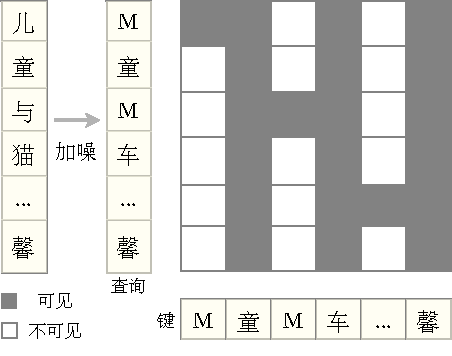
\includegraphics[width=0.6\linewidth]{figures/ddcap-attn.pdf}
  \caption{DDCap方法集中注意力掩码模块示意图}
  % image encoder; decoder (cross-attn) + time step
  \label{fig:ddcap-attn}
\end{figure}

\paragraph{集中注意力掩码模块} 前文分析指出,文本信号的离散特性导致在加噪过程中被转换为掩码标记[\texttt{MASK}]的文本标记除了作为占位符外无法提供有用信息。这一问题在训练过程加噪步数$t$较大时或推理阶段初期尤为严重。因为此时输入文本序列噪声强度大,大部分标记由掩码标记组成,所以对其他文本标记的学习造成了干扰。
% 前文分析到由于文本信号具有离散特性,若在加噪过程中某一文本标记被转换为掩码标记[\texttt{MASK}],那么该文本标记除了作为一个占位符以外无法对其他文本标记的预测提供任何有用信息。
% 这一问题在训练过程加噪步数$t$较大时,或者在推理过程的开始阶段尤为严重,因为此时输入的文本序列大部分内容由这种掩码标记组成,反而对其他正常文本标记造成干扰。

为解决此问题,DDCap方法提出集中注意力掩码模块方法。该方法通过修改注意力掩码控制模型的注意力分布,使所有位置的标记主要关注信息丰富的位置。如图\ref{fig:ddcap-attn}所示,在集中注意力掩码模块设计中,正常文本标记在自注意力机制中仅与其他正常文本标记交换信息,不与信息匮乏的掩码标记交互;而掩码标记之间也不互相影响,只从自身和正常文本标记中收集预测所需信息。这种集中注意力掩码模块提高了有噪声文本序列中有效信息间的交互效率,避免了无效信息干扰。实验表明,这种新颖的注意力掩码设计显著提升了图像描述生成任务性能。

% 为了解决这个问题,DDCap方法提出集中注意力掩码模块设计,通过修改注意力掩码来对模型注意力位置进行控制,使得所有位置的文本标记主要关注有信息量的位置。
% 如图\ref{fig:ddcap-attn}所示,对于正常文本标记而言,它在模型自注意力机制中只与其他正常文本标记进行信息交换,而不与信息含量极低的掩码标记进行交互,而对于掩码标记而言,它们之间也不会互相影响,而是主要从有信息量的正常文本标记中收集可用于自身预测的信息。% \todo{这里可以配一个图}, 对ablation里的说明也有好处。
% 通过这种集中注意力掩码的方式,DDCap方法增强了有噪声文本序列中有效信息交互的效率,避免了无效信息的干扰。实验表明这种新颖的注意力掩码设计对图像描述生成任务的性能有较大帮助。

\paragraph{最佳优先推理策略} 推理过程中,离散扩散模型每步都会针对当前输入$x_t$应用去噪过程,给出对原始文本标记$x_0$的预测结果,并通过进一步加噪和去噪的迭代过程改进对原始文本标记的预测。为鼓励模型在推理过程中尽可能保留有用信息,DDCap方法提出最佳优先推理策略。该策略在每个去噪步$t$中均会保留一定比例模型置信度高的文本标记预测结果,防止其被重新加噪,为后续生成提供更多有效信息。
具体而言,设$N_{L}$为长度预测任务给出的待生成文本序列长度。若$N_{L}\le T$,则推理过程总步数从加噪步$T$减至序列长度$N_{L}$,从而在推理过程中的每步保留置信度最高的一个文本标记。若$N_{L}>T$,则在去噪步$t$时保留$K^{t}$个置信度最高的文本标记不被重新加噪。$K^{t}$的计算方法为:
\begin{equation}
    K^{t} = \lfloor \frac{T-t+1}{T}\times N_{L}\rfloor-\lfloor \frac{T-t}{T}\times N_{L}\rfloor.
\end{equation}

% \paragraph{最佳优先推理策略} 在推理过程中,去噪网络每一步都会给出对原始文本标记序列$x_0$的预测结果,并逐渐通过进一步加噪和去噪来改进这一预测,使其更加准确。为了鼓励模型在每步推理中尽可能保留有用的信息,DDCap方法提出了一种最佳优先推理策略,使得模型在推理过程的每一个去噪步中均保留一定比例置信度较高的文本标记不被重新加噪,而这些文本标记可以为下一步生成提供有用信息。
% 具体而言,设$N_{L}$为长度预测任务给出的待生成文本标记序列长度。如果$N_{L}\le T$,则推理过程总步数会从$T$步减少到$N_{L}$步,这样在推理过程中每一个去噪步都会保留预测出来的文本序列中置信度最高的一个文本标记。
% 同时,自适应层范数中使用的阶跃索引 t 也按比例缩小。% 对于t的处理细节可以先不提
% 如果长度预测任务给出的预测长度$N_{L}$大于训练时的总加噪步数$T$,那么最佳优先推理策略会在每一个去噪步$t$中保持$K^{t}$个置信度最高的文本标记不被重新加噪。$K^{t}$的计算方法如下:
% \begin{equation}
%     K^{t} = \lfloor \frac{T-t+1}{T}\times N_{L}\rfloor-\lfloor \frac{T-t}{T}\times N_{L}\rfloor.
% \end{equation}
\paragraph{无图像引导文本生成训练策略} 图像描述生成质量受模型两个关键能力的影响,一方面是模型将视觉表征转化为文本的能力,另一方面是模型对语言信号的建模能力。受图像生成方法中的无分类器引导方法\cite{glide, VQ-diffusion}启发,DDCap方法引入无图像引导文本生成训练策略。该策略通过在训练过程中将部分图像描述任务转化为纯文本生成任务,增强了扩散模型对语言信号本身的建模能力。
具体而言,在训练过程中,无图像引导文本生成训练策略以概率$r$将CLIP视觉表征替换为可训练的随机特征$e$,指示模型学习纯文本生成任务。此时损失函数修改为:
\begin{align}
    \mathcal{L}' = -\log p_{\theta_t}({x}_{0} | {x}_{t}, {e}).
\end{align}

% \paragraph{无图像引导文本生成训练策略} 图像描述生成任务受模型两个关键能力的影响,一方面是模型将视觉表征转化为文本表征的能力,另一方面则是模型对语言建模的能力。为了增强扩散模型对语言信号本身的建模能力,受无分类器引导的图像生成方法\cite{glide, VQ-diffusion}启发,DDCap方法在图像描述生成任务中使用了类似的无图像引导文本生成训练策略,在训练过程中将一定比例的训练任务转化为不基于图像条件的纯文本生成任务。具体来说,在训练过程中,CLIP方法的视觉模型输出的视觉表征以一定的概率$r$被替换为一个可训练的随机特征$e$,来指示模型此时需要学习一个纯文本生成任务:$p_{\theta_t}(x_{0} | x_{t}, e)$。此时,模型的损失函数对应修改为:
% \begin{align}
%     \mathcal{L}' = -\log p_{\theta_t}({x}_{0} | {x}_{t}, {e}).
% \end{align}
通过无图像引导文本生成训练策略,模型能更专注于学习文本生成任务本身,增强了其语言建模能力。在推理过程中,模型可在有图像条件与无图像条件的文本描述输出间进行插值,从而控制生成的图像描述对图像的依赖程度。外推该插值函数可以增强图像描述生成过程对图像内容的关注程度,从而达到增强生成效果的目的,概率分布计算如下:
% 通过引入无图像引导的训练方法,模型可以更专注于学习如何生成文本内容,并增强其对语言建模的能力。在推理过程中,模型可以在有图像条件的文本生成和无图像条件的文本生成两种不同情况的输出间进行插值,以控制图像描述生成过程对图像的依赖程度。如果将插值过程外推,可以取得增强图像描述生成能力的效果,对应的概率分布计算如下:
\begin{equation}
    \log p_{\theta_t}({x}_{0} | {x}_{t}, {y})'=\log p_{\theta_t}({x}_{0} | {x}_{t}, {e}) + \\ s(\log p_{\theta_t}({x}_{0} | {x}_{t}, {y}) - \log p_{\theta_t}({x}_{0} | {x}_{t}, {e})),
\end{equation}
其中$s$表示图像描述生成过程对图像信息的依赖程度,$s=0$时退化为纯文本生成任务,也即不依赖CLIP视觉表征的图像描述生成任务。通常$s$的取值范围为$[1, +\infty)$:$s=1$时等价于标准图像描述生成过程,而$s>1$时模型加强对视觉表征的关注,此时通常可以得到更佳的描述生成效果。在实验中,$s$的取值略大于1。
% 其中$s$表示图像描述生成过程中对图像信息的依赖程度,当$s=0$时回退为纯文本生成任务。通常而言$s$的取值范围为$[1, +\infty)$。当$s=1$时,插值结果等价于标准图像描述生成任务的输出结果,而当$s>1$时,模型将加强对视觉表征的关注程度,此时往往会取得更佳的描述生成效果。在实验中,$s$的取值略大于1。


\section{实验结果}
\label{sec:ddcap-result}
\subsection{实验设置}
\label{sec:ddcap-exp-setting}
% CLIP模型预训练过程将大规模的图像特征与文本特征进行对齐,因此CLIP预训练得到的文本模型以判别能力为主,不适合图像注释这类文本生成任务,同时原始文本模型中没有交叉注意力模块,无法基于图像特征进行生成。
本节实验从OpenAI CLIP模型\cite{radford2021learning}出发,随机初始化用于文本生成任务迁移的离散扩散模型参数,并在CLIP-Base和CLIP-Large两个不同大小的视觉模型上进行了实验验证。
为了充分训练随机初始化的离散扩散模型,使其能更好地把CLIP视觉表征转化为文本输出,本节引入两个阶段的图像描述任务训练。第一阶段使用一个较大规模的图文数据集对新初始化的离散扩散模型进行训练,第二阶段则在MSCOCO图文数据集上进行微调并测试。为节约计算开销,消融实验只包含了第二阶段。

\paragraph{第一阶段训练设置} 按照通常的做法\cite{uniter, meter},本节将MSCOCO\cite{chen2015microsoft}、Conceptual Captions\cite{sharma-etal-2018-conceptual}、SBU\cite{sbu}和Visual Genome\cite{krishna2017visual}四个数据集中的所有图文数据对合并,构建了一个包含大约400万张图像和1000万个相关文本的通用数据集作为这一阶段的训练数据。
此阶段训练的主要超参数设置如下:使用峰值学习率为1e-4的线性衰减学习率调度,设置批大小为1024并训练了15轮次。在此阶段中,CLIP方法的视觉模型以一个更小的学习率一起训练,从而进一步增强其视觉表征的表达能力。% 最长注释长度为$20$

\paragraph{第二阶段训练设置和评测方法} 
这一阶段中使用主流的MSCOCO图文数据集进行训练和测试。MSCOCO图文数据集共包含12万张图像,每张图像配有5条图像描述。遵循通常的训练集、验证集和测试集拆分方法\cite{karpathy2015deep},该阶段使用其中的11万图像和对应的描述集合进行训练,并利用另外5000张图像进行验证,最终在剩余的5000张图像上测试模型的图像描述生成效果。
由于语义生成任务不存在标准答案,本节实验使用常见文本生成评测指标进行测试,比对了模型输出与参考描述间的相似性。本节实验使用的指标为CIDEr-D\cite{cider}、BLEU@4\cite{bleu}、METEOR\cite{meteor}、ROUGE-L\cite{rouge}和SPICE\cite{spice},从单词匹配度、公共子序列长度、语义相似性等方面对模型输出的质量进行评测。在后续实验中,这些指标被分别简称为“C”、“B@4”、“M”、“R”和“S”。
% 不同指标说明:https://juejin.cn/post/7412894237019389991

此阶段训练的主要超参数设置如下:使用峰值学习率为2e-4的线性衰减学习率调度,设置批大小为512并训练30轮次。若模型经过第一阶段的训练,则在此阶段中对模型使用1e-5的峰值学习率进行微调。% 最长注释长度为$20$

\subsection{针对关键设计的消融实验}
本节的所有消融实验使用第二阶段进行训练并在MSCOCO数据集的验证集中进行测试。为了降低计算成本,此阶段CLIP方法的视觉模型不会进行更新。%,以单独评价不同设计方法在语义生成任务上的迁移性能优劣。

\begin{table}
  \centering
  \caption{DDCap方法针对文本信号特性关键设计的消融实验}
  \begin{tabular}{lccccccccc}
    \toprule   
    序号  & 推理 & 掩码 & 长度 & 无图像引导 & C & B@4 & M & R & S \\    
    \midrule
    \#1  &&&&& 20.6 & 7.4  & 18.8 & 34.6 &12.3  \\ 
    \#2  &&$\checkmark$&&& 43.6 & 11.4  & 20.5 & 39.1 & 14.4  \\ 
    \#3   &$\checkmark$ &&&& 45.2 & 20.3  & 26.9 & 47.3 & 21.3  \\
    \#4 &$\checkmark$&&$\checkmark$& & 92.6 & 27.3  & 25.4 & 51.8 & 18.7\\
    \#5  &$\checkmark$&$\checkmark$&&& 97.5 & 28.2  & 28.1 & 54.0 & \textbf{21.7} \\
    \#6  &$\checkmark$&$\checkmark$&$\checkmark$&& 116.7 & 34.6  & 28.1 & 57.4 & 21.5\\
    \#7 &$\checkmark$&$\checkmark$&$\checkmark$&$\checkmark$& \textbf{117.8} & \textbf{35.0}  & \textbf{28.2} & \textbf{57.4} & \textbf{21.7}\\
    \bottomrule
  \end{tabular}
  \label{tab:ddcap-component}
\end{table}

\paragraph{关键设计的消融} 
\label{sec:ddcap-exp-abl}
如第\ref{sec:ddcap-key-design}节所述,DDCap方法引入以下四种设计来增强离散扩散模型在图像描述生成任务上的效果:长度预测任务(简称为“长度”)、集中注意力掩码模块(简称为“掩码”)、最佳优先推理策略(简称为“推理”)和无图像引导文本生成训练策略(简称为“无图像引导”)。

表\ref{tab:ddcap-component}展示了四种关键设计形成各类组合的消融实验,其中序号\#1实验作为基准,不使用任何针对文本信号特性的设计。实验结果表明不引入任何针对性设计的离散扩散模型无法有效实现CLIP方法的语义生成任务迁移。对比序号\#3和\#1的实验结果,可以看出应用最佳优先推理策略将CIDEr-D分数从20.6提高到45.2,说明在推理过程中保留有用信息,使其不被重新加噪的重要性。

通过对比序号\#5和\#3的实验结果,可以看出集中注意力掩码模块对文本生成离散扩散模型的重要性。引入集中注意力掩码模块后,CIDEr-D分数从45.2进一步跃升到97.5。这一现象说明集中注意力掩码模块通过对低信息量的掩码标记进行特殊处理,对模型建模去噪过程产生了明显的积极影响。% 这一点正是由文本信号的离散性和信息紧致性特点导致的。

通过对比序号\#6和\#5的实验结果,可以看出长度预测任务对图像描述生成效果的影响。引入长度预测任务有助于模型做好提前规划,并增强其判断何时终止生成文本序列的能力。相比于序号\#5的实验,该设计将模型的CIDEr-D分数提高了近20点,表明此时模型生成的图像描述在语义上与参考描述更接近。但这种方法不影响模型对语法词序等内容的建模能力,因此METEOR指标没有变化。

最后,对比序号\#7和\#6的实验结果说明无图像引导文本生成训练策略对模型性能也有一定的提升。考虑到这种方式不会带来额外的训练开销,因此DDCap方法中默认使用了此项设计。
% \todo{既然前面说了什么各种字符匹配、语义匹配的评测维度,这里也可以加下不同策略的提升方面}


\begin{table}
  \centering
  \caption{DDCap方法对集中注意力掩码模块的消融实验}
  \begin{tabular}{lccccccc}
    \toprule
    方法  & M2M & T2M & C & B@4 & M & R & S\\
    \midrule
    DDCap &$\checkmark$&$\checkmark$& 92.6 & 27.3  & 25.4 & 51.8 & 18.7  \\ 
    DDCap &$\checkmark$&& 94.1 & 27.2  & 25.7 & 52.1 & 18.9  \\ 
    DDCap  & &$\checkmark$& 115.6 & 34.2  & 27.9 & 57.2 & 21.4  \\
    DDCap  && & \textbf{116.7} & \textbf{34.6}  & \textbf{28.1} & \textbf{57.4} & \textbf{21.5}\\
     \midrule
    DDCap($t < T/2$) &&& 98.8 & 29.8  & 25.2 & 52.8 & 19.4\\
    DDCap($t\geq T/2$)  &&& 112.9 & 33.2  & 27.9 & 56.5 & 21.2\\
    \bottomrule
  \end{tabular}
  \label{tab:ddcap-maskatten}
\end{table}

\paragraph{进一步理解集中注意力掩码模块的设计} 表\ref{tab:ddcap-component}中的消融实验展示了集中注意力掩码模块对图像描述生成任务性能的增强效果。在第\ref{sec:ddcap-method}节方法介绍中提到,这一模块设计的出发点是为了减少低信息量的掩码标记对其他正常文本标记的信息获取能力造成影响。该模块主要通过两部分设计修改了模型内部的信息交换机制:1)正常文本标记不从掩码标记中接收信息;2)掩码标记之间不交换信息。为了进一步理解文本生成离散扩散模型内的最优信息流动机制,表\ref{tab:ddcap-maskatten}中引入如下四种设置:
\begin{itemize}
    \item “M2M”意为允许掩码标记之间互相交换信息。
    \item “T2M”意为允许正常文本标记从掩码标记中获取信息。
    \item “$t < T/2$”意为对$t$较小的加噪步中应用集中注意力掩码模块。此时输入文本序列中掩码标记的比例较低。
    \item “$t\geq T/2$”意为对$t$较大的加噪步中应用集中注意力掩码模块。此时输入文本序列中的掩码标记比例较高。
\end{itemize}
 
表\ref{tab:ddcap-maskatten}展示了不同信息流动机制对模型性能的影响。实验发现,禁止掩码标记之间互相交换信息与禁止正常文本标记从掩码标记中获取信息两种方式都对模型性能有明显帮助,其中前者设计对模型性能有更显著的影响。造成这一现象的原因是,在离散扩散模型中掩码标记本身仅起到占位符的作用,而不同占位符之间除位置编码略有不同之外,内部表征非常相似。这种相似性可能会使得模型将不同位置的掩码标记混淆,从而导致错误的预测结果。此外,因为掩码标记本身信息含量很低,所以允许正常文本标记从掩码标记中获取信息并不会对该文本标记的预测有帮助。因此,文本生成离散扩散模型的最优信息流动方向应该是从高信息的正常文本标记流向其他正常文本标记或低信息的掩码标记。

与此同时,通过对比在低噪声训练步或高噪声训练步中引入集中注意力掩码模块的两组实验结果表明,在高噪声训练步中引入该方法对性能提升更加显著。因为此时输入文本序列中的掩码标记比例更高,所以模型更容易出现不同掩码标记间混淆的情况。这一结果也验证了对文本生成离散扩散模型内最优信息流动方向的猜测。

\begin{figure}
  \centering
  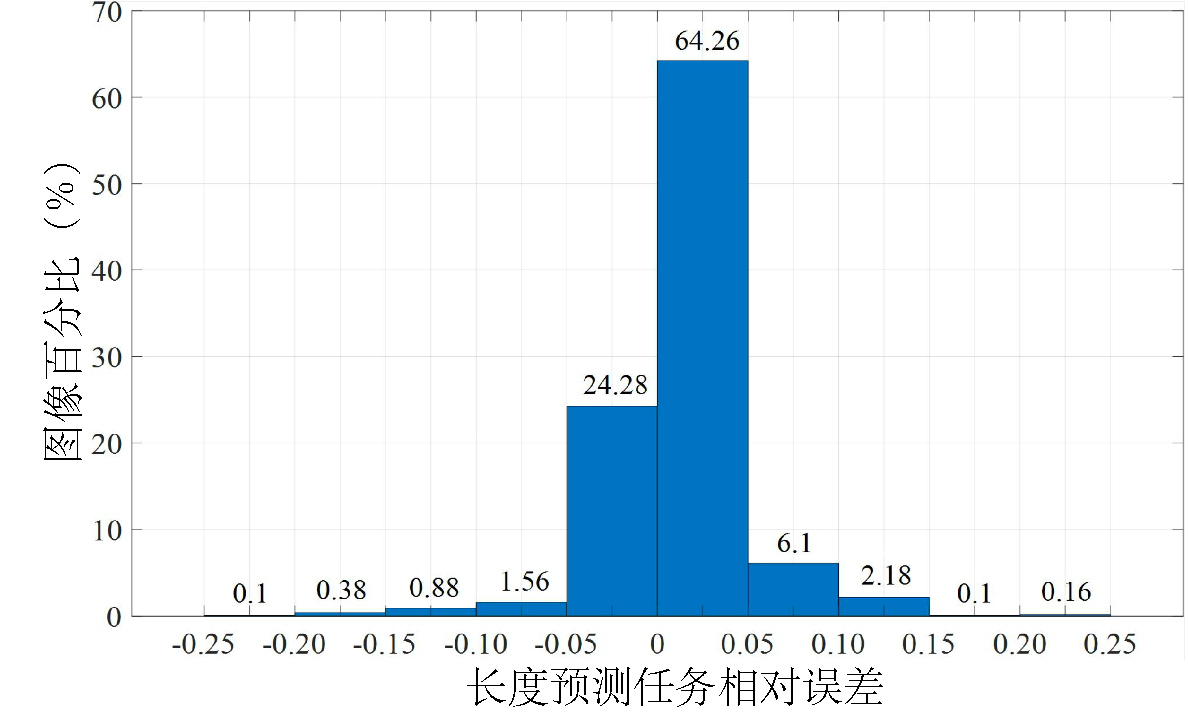
\includegraphics[width=0.7\linewidth]{figures/ddcap-length.pdf}
  \caption{DDCap方法长度预测任务的相对误差分布}
  % image encoder; decoder (cross-attn) + time step
  \label{fig:ddcap-length}
\end{figure}

\paragraph{长度预测任务的准确率} 图\ref{fig:ddcap-length}展示了DDCap方法在长度预测任务上的相对误差分布。相对误差的计算方式为$(N_{L}-N_{G})/N_{G}$,其中$N_{L}$表示模型预测的序列长度,$N_{G}$为实际序列长度。
% \todo{每个图像有5个注释文本,这玩意儿是咋测的} 是training统计吗?
统计结果表明有90\%的图像描述序列长度预测误差率在5\%以内。考虑到实验中最大序列长度为20,5\%的相对误差对应着误差一个文本标记,因此该长度预测任务的准确率在可接受范围内。

\begin{table}
  \centering
  \caption{DDCap方法中不同时间信息嵌入方式的对比实验}
  \begin{tabular}{lcccccc}
    \toprule
    方法 & $\text{step}_{\text{Scale}}$ & C & B@4 & M & R & S\\
    \midrule
    无信息嵌入 & - & 115.5 & 34.2  & 28.0 & 57.3 & 21.3\\
    自适应层归一化嵌入 & - & 115.1  & 34.1 & 28.0 & 57.1 & 21.3\\
    正余弦位置嵌入 & 4000 & 115.9 & 34.5  & 28.0 & \textbf{57.4} & 21.4\\
    正余弦位置嵌入 & 6000 & 114.8  & 33.7  & 27.9 & 57.0 & \textbf{21.5}\\
   正余弦位置嵌入 & 8000 & \textbf{116.7}  & \textbf{34.6}  & \textbf{28.1} & \textbf{57.4} & \textbf{21.5}\\
   正余弦位置嵌入 & 10000 & 115.1  & 34.0  & 27.9 & 56.9 & 21.3\\
    \bottomrule
  \end{tabular}
  \label{tab:ddcap-adaptivet}
\end{table}

\paragraph{去噪步时间信息嵌入方式的对比实验} 
在第\ref{sec:ddcap-method-all}节方法介绍中提到扩散模型在不同的去噪步$t$下会表现出不同的模型行为,以实现对不同噪声强度的自适应处理。如公式\eqref{eq:ddcap-t}所示,DDcap方法使用正余弦位置嵌入方法将去噪步信息传入到模型中。
表\ref{tab:ddcap-adaptivet}展示了正余弦位置嵌入方法与不引入去噪步时间信息的基线以及自适应层归一化嵌入方法的比较结果。结果表明,适当调整正余弦位置嵌入方法的$\text{step}_{\text{scale}}$值可以在一定程度上提升CLIP方法在图像描述生成任务上的迁移性能。将$\text{step}_{\text{scale}}$设为0时,实验结果与不引入去噪步时间信息的基线等价。实验表明适当区分不同去噪步间的模型行为对图像描述生成任务性能有一定帮助。

% \paragraph{无图像训练} 超参数(即r 和 s)的影响如图 4 所示。当训练比率 r 为 0.2 且推理量表为 1.17 时,我们的模型取得了最佳性能。值得注意的是,最佳指导比例范围与通常设置为 5 的图像生成范围不同 [64]
\begin{table}
  \centering
  \caption{CLIP方法与其他预训练方法在语义生成任务上的迁移性能比较}
  \begin{tabular}{lccccc}
    \toprule
    视觉预训练方法  & C & B@4 & M & R & S\\
    \midrule
    DINO & 99.3  & 29.6 & 25.9 & 53.6 & 19.3 \\
    DeiT & 100.7 & 29.6 & 25.9 & 53.9 & 19.5 \\
    CLIP  & \textbf{117.8} & \textbf{35.0} & \textbf{28.2} & \textbf{57.4} & \textbf{21.7}\\
    \bottomrule
  \end{tabular}
  \label{tab:ddcap-cmp-clip}
\end{table}

\paragraph{CLIP方法与其他预训练方法在语义生成任务上的迁移性能比较}
表\ref{tab:ddcap-cmp-clip}中展示了CLIP方法的视觉模型与其他主流视觉模型在语义生成任务上的迁移性能对比。实验结果表明,CLIP方法在图像描述生成任务上的表现明显优于DINO\cite{dino}和DeiT\cite{deit}等自监督或图像分类预训练方法。在CIDEr-D指标上,CLIP方法达到了117.8的得分,比DINO和DeiT分别高出18.5和17.1;在BLEU@4指标上,CLIP方法也获得了35.0的较高分数,明显优于其他两种方法。这一结果充分证明了CLIP方法通过语言-图像对比学习获取的视觉表征,对语义生成任务具有显著优势。这是因为CLIP方法在预训练阶段已经学习了图像与文本之间的语义对应关系,所以模型能够更准确地将视觉表征映射到相应的文本描述,为语义生成任务奠定了良好基础。

\begin{figure}
  \centering
  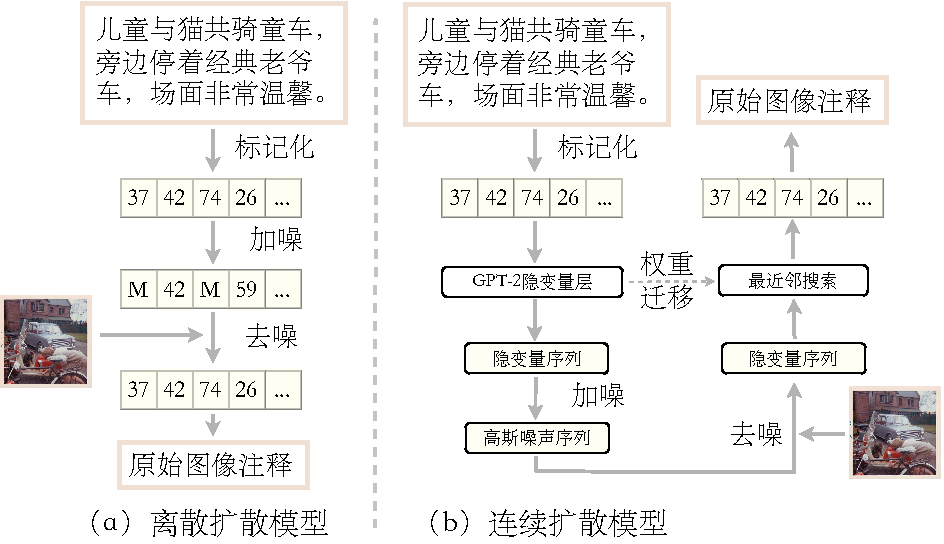
\includegraphics[width=0.8\linewidth]{figures/ddcap-cmp-continuous.pdf}
  \caption{文本生成离散扩散模型与连续扩散模型的建模方式对比}
  % image encoder; decoder (cross-attn) + time step
  \label{fig:ddcap-cmp-continuous}
\end{figure}

\subsection{与其他文本生成迁移方法的比较}
本节实验将离散扩散模型DDCap与连续扩散模型以及传统的自回归方法进行了比较。与连续扩散模型相比,离散扩散模型更符合文本信号特性,因此在图像描述生成任务中表现更优。而与传统的自回归方法相比,离散扩散模型允许对上下文同时进行建模,也可以取得相对更佳的表现。引入两阶段训练过程后,DDCap方法在图像描述生成任务中可以达到与一些大规模自回归生成方法相当的表现,并显著优于已有的非自回归方法。

\paragraph{与连续扩散模型和自回归方法的对比} 
本节实验设置与第\ref{sec:ddcap-exp-abl}节中的消融实验设置保持一致,只使用第二阶段数据进行训练和测试,并保证不同方法之间使用的生成模型参数量一致,以便公平比较。连续扩散模型和自回归方法的设置如下:
\begin{enumerate}
    \item 连续扩散模型用于文本生成任务的设计受图像生成领域中隐变量扩散模型\cite{latentdiff}启发。隐变量扩散模型本质是利用一个已训练好的隐变量提取器将连续或离散的输入信号转化为连续的隐变量,然后应用连续扩散模型进行建模。
    将该思想应用于文本生成任务时,本实验利用GPT-2预训练模型作为隐变量提取器,把离散的文本标记序列转换成连续的隐变量序列,并使用高斯噪声进行加噪过程。连续扩散模型的训练目标是基于加噪后的隐变量序列预测原始隐变量序列,再利用GPT-2预训练模型通过最近邻搜索恢复出原始文本标记。整体流程如图\ref{fig:ddcap-cmp-continuous}所示。
    %总步长 T 的数目设置为 10,000,并且噪声计划是线性的。
    % 我们发现它有助于以下修改:1) 使用所有 em 的均值和方差归一化嵌入层层理向量;2) 在推理过程中,每个嵌入向量 $x_{t}$ 被解码为标记,然后重新嵌入到向量中,然后估计 $x_{t-1}$ 。
    \item 自回归方法的设置与通常做法类似:在给定CLIP视觉表征之上训练一个自回归解码器以实现文本生成任务,并和DDCap方法一致,通过交叉注意力的机制将视觉表征引入自回归解码器中。
\end{enumerate}

\begin{table}
  \centering
  \caption{DDCap方法与连续扩散模型和自回归方法的性能对比}
  \begin{tabular}{lccccc}
    \toprule
    方法  & C & B@4 & M & R & S\\
    \midrule
    自回归方法 & 112.8  & 33.9 & 28.0 & 56.4 & 21.3\\
    连续扩散模型 & 91.9 & 25.0 &25.0&51.1& 19.1 \\
    DDCap  & \textbf{117.8} & \textbf{35.0}  & \textbf{28.2} & \textbf{57.4} & \textbf{21.7}\\
    \bottomrule
  \end{tabular}
  \label{tab:ddcap-framecom}
\end{table}
% 将连续扩散模型的训练轮次加长到100个
实验结果如表\ref{tab:ddcap-framecom}所示。与连续扩散模型相比,离散扩散模型在图像描述生成任务上的表现明显更优。这是因为离散扩散模型利用了文本信号具有离散性、冗余性低等特点,所以更适合以文本生成为目标的图像描述生成任务。
与自回归方法相比,离散扩散模型的表现也更优。这可能是由于离散扩散模型模拟了人类写作过程中的修正策略,允许模型在推理过程中利用上下文信息对中间文本标记进行修改,因此避免了因固定生成顺序而导致的误差累积问题。

\paragraph{与大规模自回归方法和其他非自回归方法的对比} 参照大规模自回归方法的训练策略,本组实验在DDCap方法中引入了第一阶段的通用图文数据集进行训练,并在第二阶段中针对MSCOCO数据集进行微调。表\ref{tab:ddcap-compsota}展示了DDCap方法与大规模自回归方法和其他非自回归方法的比较结果。
% 其中标注了$^\dagger$的方法引入了额外的目标检测模型对视觉表征进行增强。% \todo{把这些数据单位统一下,没有的数字要确认} 特别是那些别的单位的
与其他非自回归方法相比,DDCap方法取得了最佳性能,表明了新方法的有效性。% 可能要看一下和之前非自回归方法的主要区别
与已有的大规模自回归方法相比,在训练图像数量相当的情况下,DDCap方法的图像描述生成性能已经优于许多已有方法,并与ViTCap\cite{ViTCap}方法表现相当。这一结果展现了利用离散扩散模型实现高质量语义生成任务迁移的潜力。


\begin{table}
  \centering
  \caption{DDCap方法与自回归方法和非自回归方法的性能对比}
  % \setlength\tabcolsep{3pt}
  \begin{tabular}{lcccccc}
    \toprule
    方法 & 参数量 & 训练图片数 & C & B@4 & M & S\\
    \midrule
    \multicolumn{7}{l}{\textbf{自回归方法}}\\
    \midrule
    $\rm{UVLP}$~\cite{zhou2020unified}  & 0.1B & 4M & 116.9 & 36.5 & 28.4 & 21.2 \\
    % $\rm{MiniVLM}$~\cite{wang2020minivlm}  & 34.5M & 14M & 119.8 &  35.6 & 28.6 & 21.6  \\
    % $\rm{DistillVLM}$~\cite{fang2021compressing}  & 34.5M & 7M & 120.8 &  35.6 & 28.7 & 22.1 \\
    $\rm{UFO_B}$~\cite{UFO} & 0.1B & 4M & 122.8 & 36.0 & 28.9 & 22.2 \\
    $\rm{OSCAR_B}$~\cite{OSCAR} & 0.2B & 7M & 123.7 & 36.5 & 30.3 & 23.1\\ 
    $\rm{UNIMO_B}$~\cite{UNIMO}  & 0.2B & 9M & 124.4 &  38.8 & - & - \\
    ViTCap~\cite{ViTCap} & 0.2B & 4M & 125.2 & 36.3 & 29.3 &  22.6 \\
    $\rm{VinVL_B}$~\cite{VinVL} &  0.3B & 6M & 129.3 & 38.2 & 30.3 & 23.6\\ 
    $\rm{GIT_B}$~\cite{GIT} & 0.1B & 4M & 131.4 & 40.4 & 30.0 & 23.0 \\
    $\rm{LEMON_B}$~\cite{LEMON}& 0.1B & 200M& 133.3& 40.3& 30.2& 23.3\\
    $\rm{SimVLM_B}$~\cite{SimVLM}& -& 1800M & 134.8& 39.0& 32.9& 24.0\\ 
    % $\rm{OFA_B}$~\cite{wang2022ofa} & 184M & 4M & 138.2 & 41.0 & 30.9 & 24.2 \\
    \midrule
    \multicolumn{7}{l}{\textbf{非自回归方法}}\\
    \midrule
        $\rm{MNIC}$~\cite{gao2019masked}  & -  & - & 108.5 & 31.5 & 27.5 & 21.1\\
    $\rm{NAIC_{B,KD}}$~\cite{guo2020non}  & -  & - & 115.5 & 35.3 & 27.3 & 20.8\\
        $\rm{FNIC}$~\cite{fei2019fast}  & -  & - & 115.7 & 36.2 & 27.1 & 20.2\\
            $\rm{DDCap}$  & 0.3B & 4M & \textbf{125.1} & \textbf{37.1} & \textbf{29.1} & \textbf{22.7}\\
    % \hline  
    % $\rm{LEMON_L}$~\cite{hu2022scaling} & 338.3M & 0.2B & 135.7 & 40.6 & 30.4 & 23.5\\
    % $\rm{SimVLM_L}$~\cite{wang2021simvlm} & - & 1.8B & 142.6 & 40.3 & 33.4 & 24.7\\ 
    % $\rm{OSCARB_L}$~\cite{li2020oscar} & 0.3B+64M & 4M & 127.8 & 37.4 & 30.7  & 23.5\\ 
    % $\rm{VinVL_L}$~\cite{zhang2021vinvl} &  0.3B+0.2B & 6M & 130.8 & 38.5 & 30.4 &  23.4\\ 
    % $\rm{UFO_L}$~\cite{wang2021ufo} & 0.3B & 4M & 131.2 & 38.7 0 & 30.0 & 23.3 \\
    % $\rm{GIT_L}$~\cite{wang2022git} & 0.3B & 14M & 138.5 & 42.0 & 30.8 & 23.8 \\
    % $\rm{OFA_L}$~\cite{wang2022ofa} & 472M & 4M & 142.2 & 42.4 & 31.5 & 24.5 \\  
    % mPLUG~\cite{li2022mplug} & 0.6B & 14M & 141.0 & 43.1 & 31.4 & 24.2 \\
    \bottomrule
  \end{tabular}
%   \caption{Performance comparison on COCO captioning Karpathy~\cite{Karpathy2017DeepVA} split with pretraining, where B@4, M, R, C denote BLEU@4, METEOR, ROUGE-L,
% CIDEr and SPICE scores. CIDEr optimization is not used for all models. ($\dagger$) VinVL/OSCAR: the extra parameters are for
% object detector. All of the results do not contain CIDEr optimization.}
  \label{tab:ddcap-compsota}
\end{table}

% 可以把FD-CLIP的结果也放进来(from zixin)
% ckpt:https://vlpretraineastus.blob.core.windows.net/exp/output/simmlim/simmim_pretrain_clipfeat_nomask_SmoothL1_afterln_3e_4__vit_base__img224__300ep_crop008_dp02/ckpt_epoch_299.pth
% 不过实验设置对得不是很齐(pre-train 15ep,哦,我们也是pt15m,只是没有ft)而且只测了C,没测其他,可能还有些别的设置不太一样
% baseline是124.42,fd之后是126.43,384是127.388

\paragraph{特征图自蒸馏方法增强语义生成任务迁移性能的比较} 在第\ref{cha:fd}中介绍了通过特征图自蒸馏方法引入细粒度视觉目标,从而取得更佳视觉任务迁移效果的实验。之前的结果主要侧重于细粒度视觉任务,比如语义分割、深度估计等,而本实验在语义生成任务上对特征图自蒸馏方法进行了测试。实验结果如表\ref{tab:ddcap-fd-clip}所示,经过特征图自蒸馏的CLIP模型在语义生成任务上也取得更佳表现,展现出了特征图自蒸馏方法对CLIP模型的全面提升。
这一结果表明,依赖密集感知能力的细粒度视觉任务和语义生成任务共享了部分对视觉模型能力的要求。

\begin{table}
  \centering
  \caption{特征图自蒸馏增强语义生成任务迁移性能的比较}
  \begin{tabular}{lc}
    \toprule
    视觉预训练方法  & C\\
    \midrule
    CLIP & 125.1 \\
    FD-CLIP & \textbf{126.4} \\
    \bottomrule
  \end{tabular}
  \label{tab:ddcap-fd-clip}
\end{table}
\subsection{图像描述修改任务与模型定性分析}



\paragraph{DDCap方法在图像描述修改任务中的表现}
由于DDCap方法是一种并行生成方法,文本标记不是从左到右按固定顺序进行生成。因此此类方法有利于处理需要对图像描述进行填充或修改的任务。
如图\ref{fig:ddcap-modification-task}所示,本节考虑了一种人机交互的应用场景,在该场景中模型需要针对人类反馈对图像描述进行修改。具体而言,该任务模拟了用户要求模型修改已生成图像描述中的形容词并返回一条新的图像描述的场景。% 本组实验通过筛选出图像注释中含有形容词的所有测试样本,并将其中的形容词去除,要求模型重新生成。
\begin{figure}
  \centering
  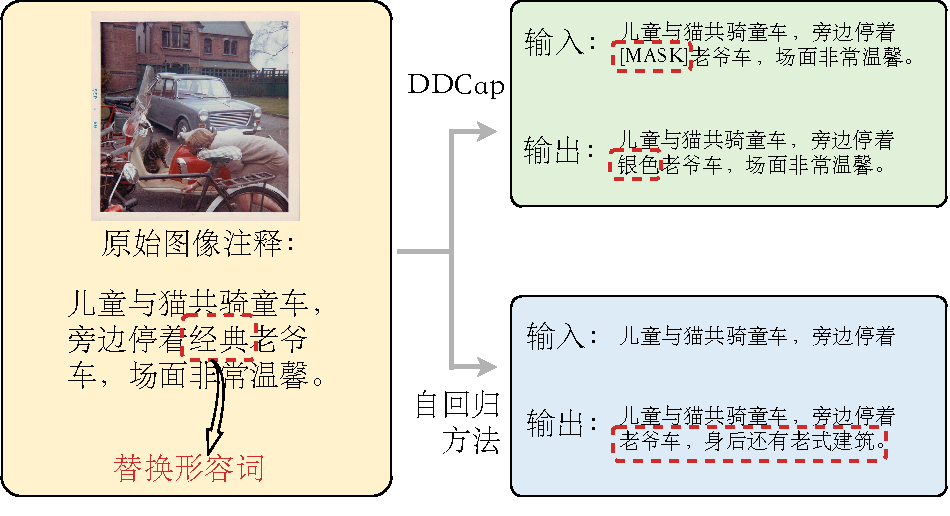
\includegraphics[width=0.8\linewidth]{figures/ddcap-modification-task.pdf}
  \caption{考虑人机互动场景的图像描述修改任务示意图}
  % image encoder; decoder (cross-attn) + time step
  \label{fig:ddcap-modification-task}
\end{figure}

表\ref{tab:ddcap-infill}展示了DDCap方法与自回归方法在图像描述修改任务上的性能比较。由于DDCap方法是一种并行生成方法,它在生成当前文本标记时能够同时考虑前文和后文。不同于自回归方法,DDCap方法可以完全保留后文而不需要重新生成。因此,DDCap方法在比较图像描述修改前后的单词匹配度、公共子序列长度等测试指标上更有优势。
为了进一步评估修改后图像描述与图像的匹配程度,本组实验引入了CLIPScore\cite{CLIPScore}指标。该指标利用CLIP模型对齐视觉表征和语言表征的能力,可以有效评估修改后图像描述与图像间的语义关系,建模单个形容词改动带来的细微语义变化。从结果来看,DDCap方法相比于自回归方法在此类图像描述修改任务上效果更佳。
\begin{table}
  \centering
  \caption{DDCap方法和自回归方法在图像描述修改任务上的对比实验}
  \begin{tabular}{lcccccc}
    \toprule
    方法 & C & B@4 & M & R & S & CLIP-Score\\
    \midrule
    自回归方法 & 203.5 & 76.3  & 49.3 &89.1& 36.5 & 75.7\\
    DDCap & \textbf{230.3} & \textbf{85.1}  &  \textbf{56.3} & \textbf{93.1} & \textbf{39.9} & \textbf{76.4}\\
    \bottomrule
  \end{tabular}
  \label{tab:ddcap-infill}
\end{table}

\begin{figure}
  \centering
  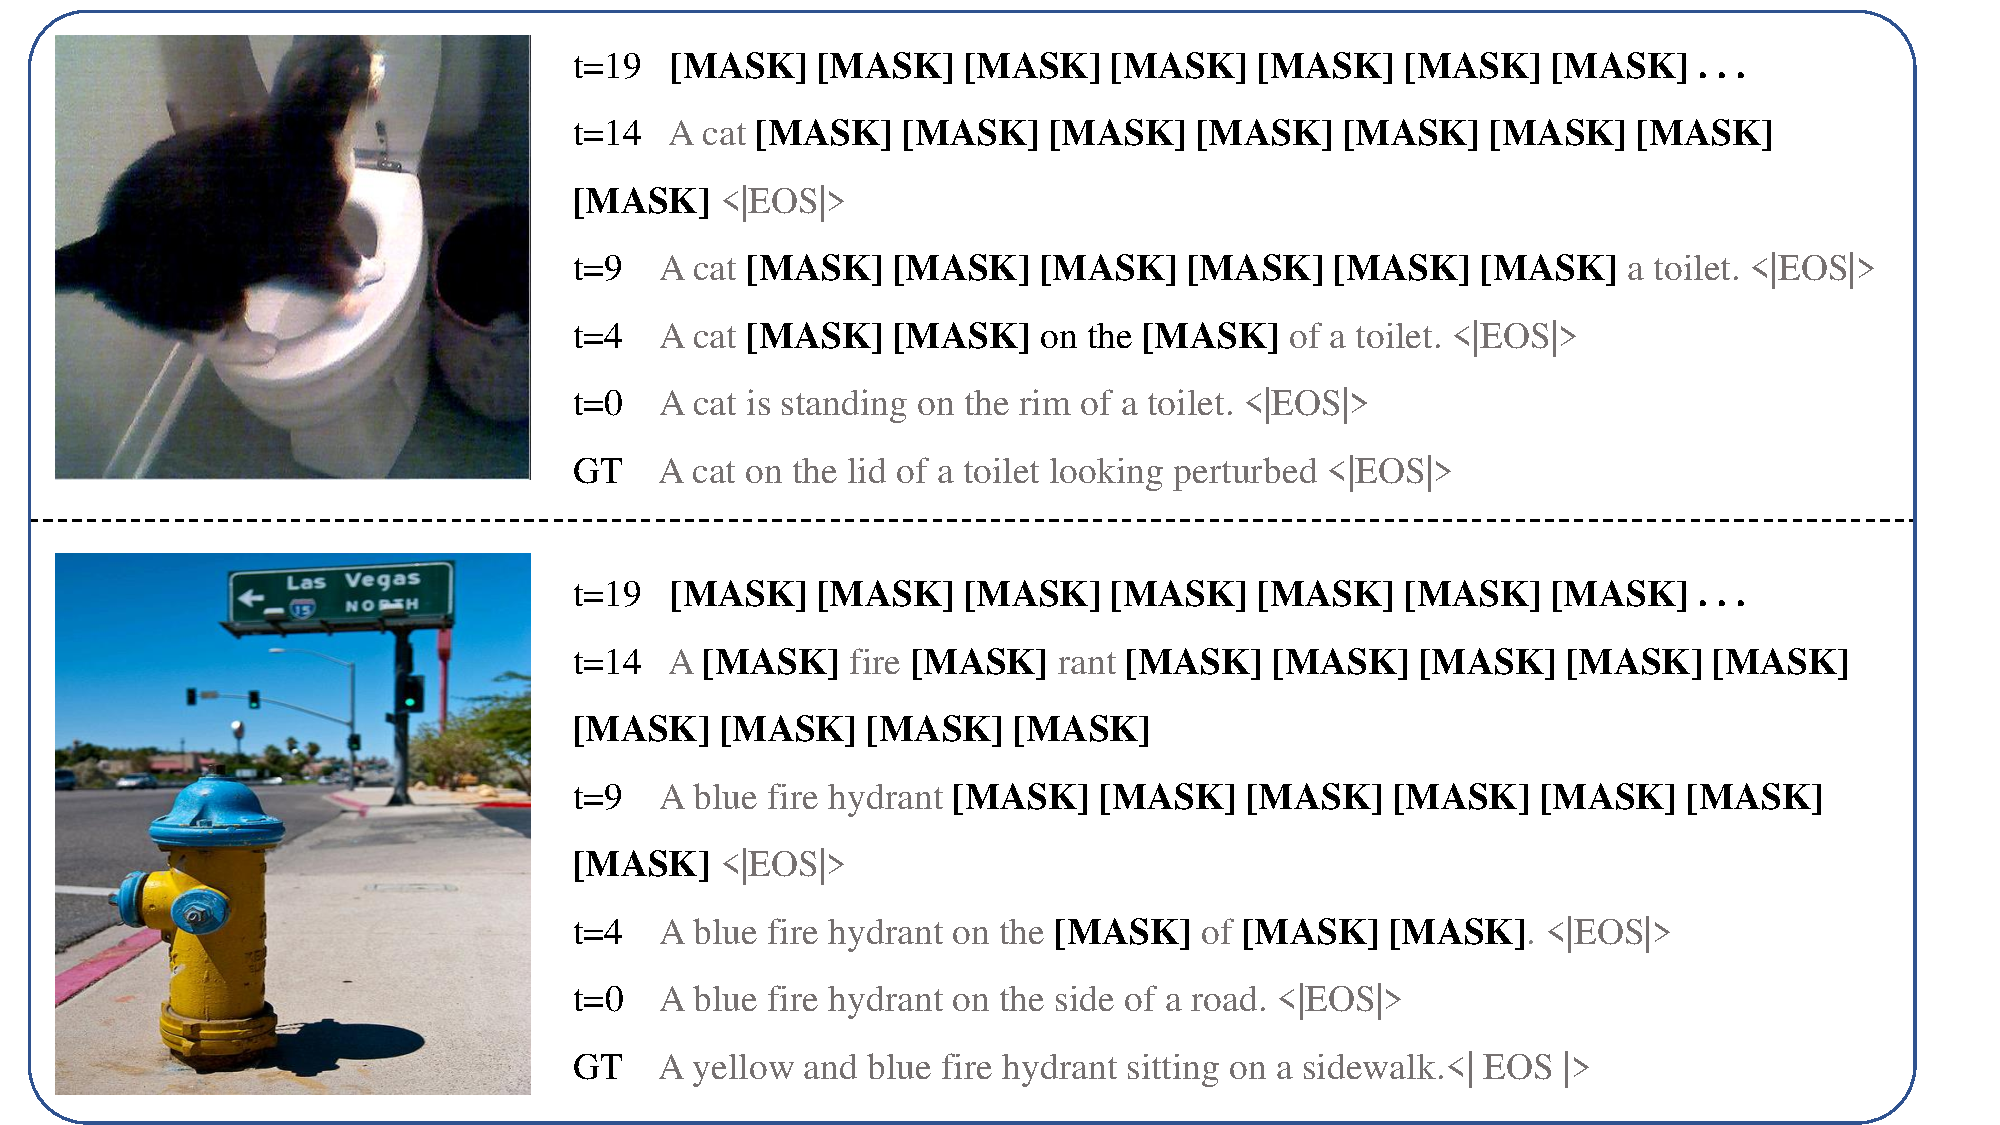
\includegraphics[width=1.0\linewidth]{figures/ddcap-generate-order.pdf}
  \caption{DDCap方法生成图像描述过程的可视化}
  % image encoder; decoder (cross-attn) + time step
  \label{fig:ddcap-generate-order}
\end{figure}



\paragraph{模型定性分析} 图\ref{fig:ddcap-generate-order}以MSCOCO测试集中的部分图像为例,展示了DDCap方法生成图像描述的顺序。通过观察模型的行为,可以得出如下结论:DDCap方法通常首先生成图像中的主体对象和对应的冠词,接着生成表示主体对象间相对关系的介词以及描述这些对象的形容词,最后生成其他名词、动词等使得句子语法正确。这一过程与人类自然思维顺序有一定相似性,展现了从点到线再到面的生成逻辑。

此外,图\ref{fig:ddcap-qualification}展示了DDCap方法和自回归方法在MSCOCO测试集部分样例上的图像描述生成结果,其中“AR”表示自回归方法生成的图像描述,而“GT”表示数据集中的参考描述。图中灰色块展示了部分生成结果的错误之处。相比于自回归方法,DDCap方法在识别图像中的主体对象方面表现更优。但由于DDCap方法依赖长度预测任务,且如图\ref{fig:ddcap-length}所示,长度预测误差存在较明显的分布倾向,也即预测序列长度比实际序列长度略长的概率更大。因此,当图像描述序列的长度预测结果更长,与实际长度有较大偏差时,DDCap方法生成的图像描述存在利用重复内容填充给定序列长度的现象。
% 但是,我们的 DDCap 有时会生成一些重复的单词。这个问题可以通过两种方式处理:(i) 我们首先获取标题,然后找到这些重复的单词。这些重复的单词将被重新屏蔽和重新生成。(ii) 标题中重复的单词将被删除。然后我们得到这个标题的新长度,没有重复的单词。根据新的长度,我们重新生成整个标题。
\begin{figure}
  \centering
  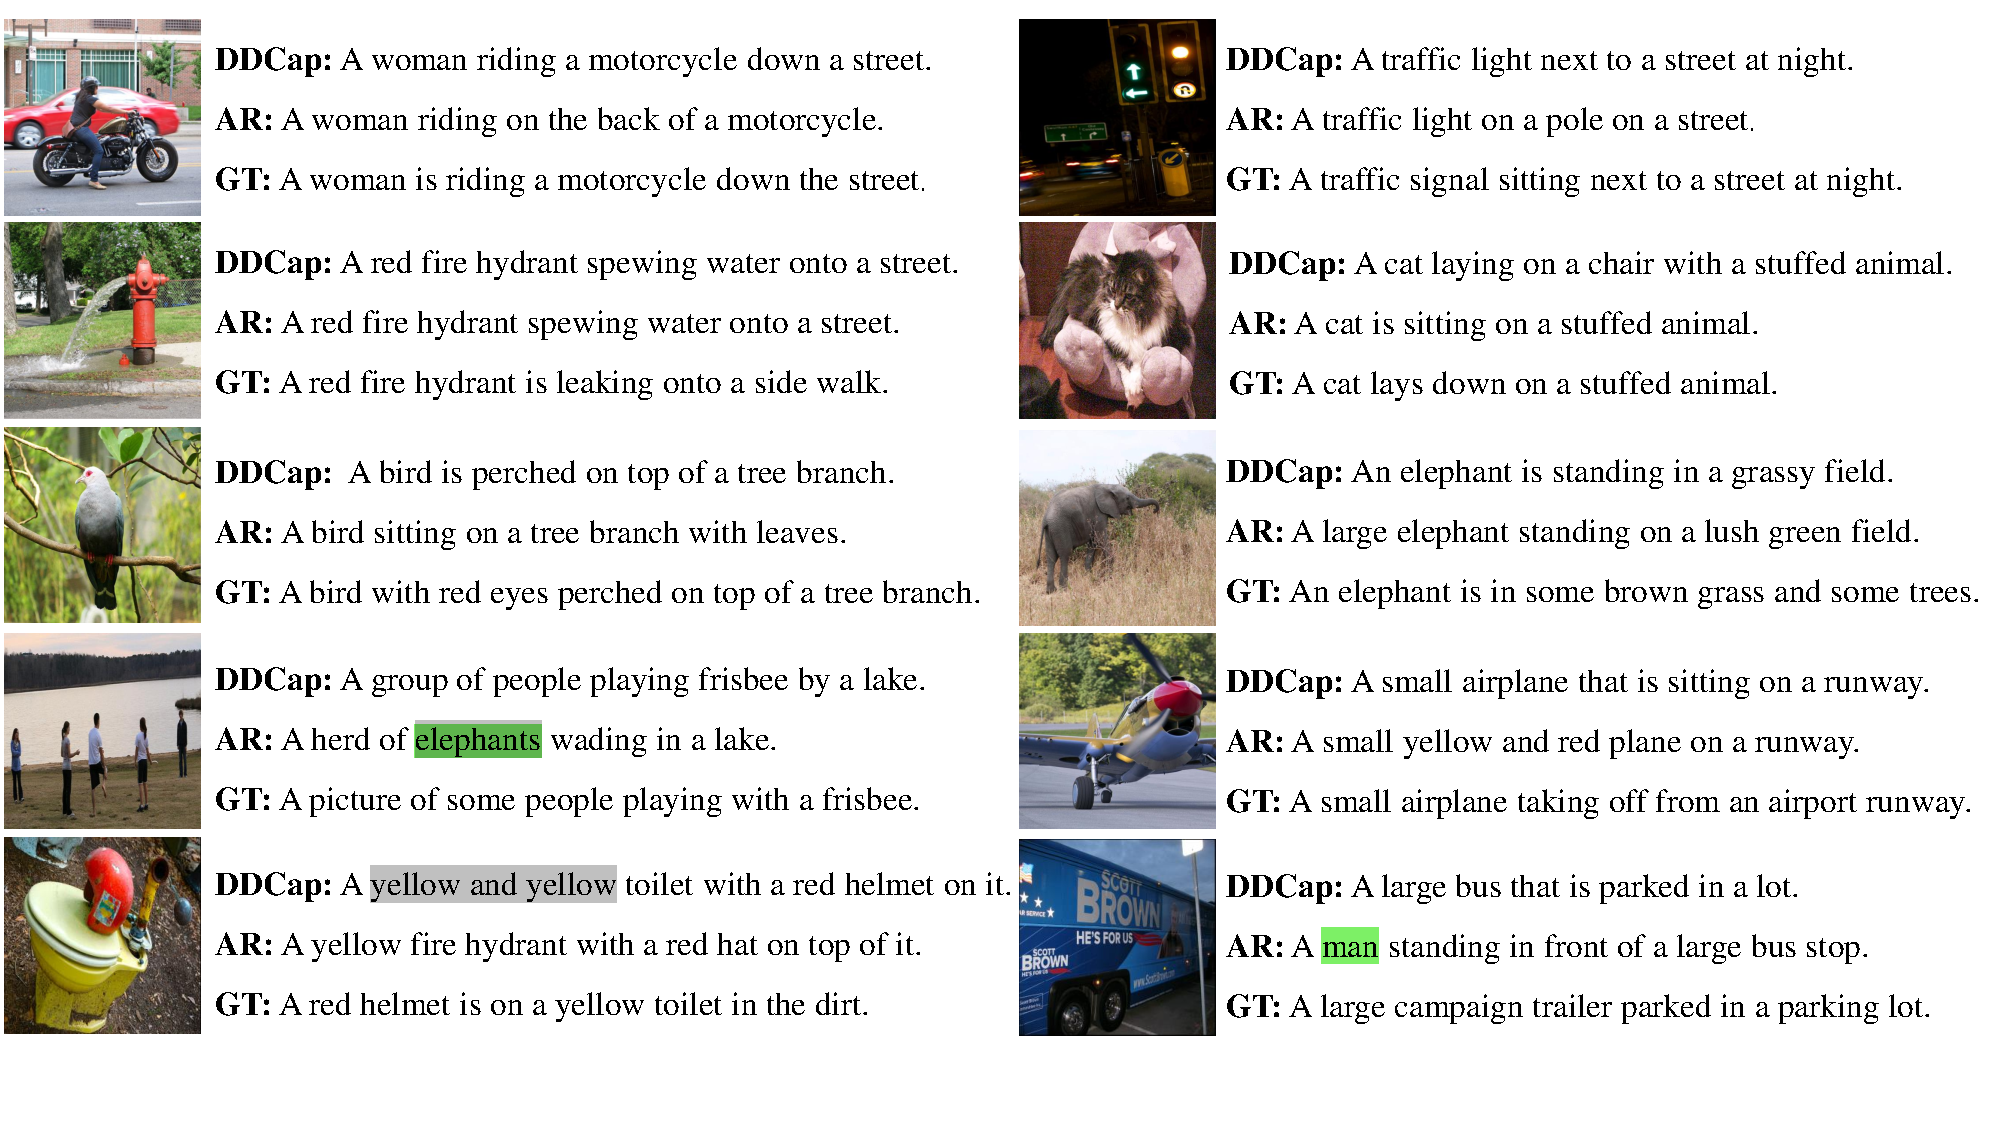
\includegraphics[width=1.0\linewidth]{figures/ddcap-qualification.pdf}
  \caption{DDCap方法与自回归方法的图像描述生成结果可视化}
  % image encoder; decoder (cross-attn) + time step
  \label{fig:ddcap-qualification}
\end{figure}

\section{总结}
\label{sec:ddcap-summary}
% \todo{怎么都没有提并行生成加速的事情?那前面里离散的motivation也别提了。}

% 因此,本文的贡献总结为
% • 我们是第一个将离散扩散模型应用于图像描述的公司,并提供了第一个证据,证明扩散模型可以达到与最好的、完善的自回归模型相比的竞争性能。
% • 我们提出了四个关键设计:(i) 长度预测用于处理文本生成中的可变长度问题;(ii) 集中注意力掩码用于提取紧凑的文本信息,而不会受到不需要的噪音的干扰;(iii) 提出了最佳优先推理以减少污染正确生成的令牌的机会;(iiii) 无图像训练,以平衡文本先验和图像条件中的信息。
% • 我们进一步展示了离散扩散模型在标题填充任务中的优势。

% 背景+motivation
语言-图像对比学习方法通过大规模互联网图文数据对训练,实现了视觉表征与语言表征的有效对齐。CLIP方法不仅增强了视觉表征的零样本泛化能力和下游视觉任务的迁移效果,还构建了多模态共享的联合表征空间,显著提高了跨模态转化效率。本章重点探讨了基于CLIP视觉表征的语义生成任务迁移方法。
% 对齐了视觉表征和语言表征。CLIP方法在增强了视觉表征的零样本泛化性和下游视觉任务迁移效果的同时,构建了两种模态共享的表征空间,极大地提升了不同模态间的转化效率。
% Dall-E 2的工作正是利用了CLIP方法搭建的跨模态桥梁,实现语言表征向视觉表征的映射,以完成基于文本的图像生成任务。受Dall-E 2的启发,
% 本章讨论了基于CLIP视觉表征实现语义生成任务的迁移方法设计。

% 解决方案和发现
受到扩散模型在图像生成任务中成功应用的启发,本章讨论了扩散模型作为图像描述生成任务迁移方法的可行性。直接将针对图像生成任务设计的扩散模型应用到文本生成任务上存在诸多问题,因此本章分析了文本信号区别于图像信号的关键特性:离散性、低冗余性、序列长度可变性。基于这些分析,本章提出了DDCap方法,通过集中注意力掩码模块、长度预测任务和最佳优先推理策略有针对性地适配文本信号特点。
% 针对文本信号离散性的特点,本章以离散扩散模型为出发点,利用不同文本标记之间的转移和作为占位符的掩码标记[\texttt{MASK}]来代替针对连续信号设计的高斯噪声。在训练过程中考虑到文本信号的变长特性,本章引入待生成注释长度预测任务,以灵活地适应不同长度的文本。同时考虑到文本信息的低冗余性,以及由标记离散性导致的噪声强度不连续性,本章提出一个集中注意力掩码模块,以引导模型关注信息密度更高的标记。
% 在推理过程设计中同样考虑了低冗余性的特点,使用一种称为最佳优先推理的策略,在每一步中保留模型置信度最高的一些标记,并只对其他标记进行重新加噪后重新生成。此外,本章还将图像生成方法中的无分类器引导思想引入文本生成任务中。该方法在训练过程中随机丢弃图像输入,以达到强制模型学习语言建模的先验知识。
% 结果
实验证明了离散扩散模型在图像描述生成任务中的有效性。与其他并行生成方法相比,DDCap方法显著缩小了与主流自回归方法间的性能差距,并在需要人机交互的图像描述修改场景中展现出独特优势。

% 针对扩散模型在图像描述生成任务中的应用,本章分析了文本信号区别于图像信号的关键特性:离散性、低冗余性和变长特性。基于这些分析,本章提出了DDCap方法,并通过实验证明了离散扩散模型在图像描述生成任务中的有效性。与其他并行生成方法相比,DDCap方法显著缩小了与主流自回归模型间的性能差距,并在需要人机交互的图像描述修改场景中展现出独特优势。

% 总结前三章工作
结合本章工作与前序两章工作,本文系统性地探讨了CLIP方法的视觉表征预训练策略和下游任务迁移方法,包括利用高质量标注的图像分类数据增强CLIP视觉表征泛化性和语义准确度、通过特征图自蒸馏提升CLIP方法细粒度视觉任务的迁移效果、以及基于离散扩散模型实现CLIP方法向语义生成任务迁移的方法。这一系列工作全面提升了CLIP方法在多种视觉和多模态任务中的应用能力。

% 结合前两章工作,本研究系统性地探讨了CLIP方法的预训练策略和下游任务迁移技术,包括利用高质量标注数据增强视觉表征泛化性、通过特征图自蒸馏提升细粒度视觉任务的迁移效果,以及基于离散扩散模型实现语义生成任务的迁移方法。这一系列工作全面提升了CLIP模型在多种视觉和跨模态任务中的应用能力。